\documentclass{sig-alternate-05-2015}
\usepackage{graphicx}
\usepackage{subfigure}
\usepackage{times}
\usepackage{balance}
\newcommand{\bi}{\begin{itemize*}}
\newcommand{\ei}{\end{itemize*}}
\newcommand{\be}{\begin{enumerate*}}
\newcommand{\ee}{\end{enumerate*}}
\newcommand{\tion}[1]{\textsection\ref{sect:#1}}
\newcommand{\fig}[1]{Figure~\ref{fig:#1}}
\newcommand{\eq}[1]{Equation~\ref{eq:#1}}
\usepackage{mathptmx} \usepackage[scaled=.90]{helvet} \usepackage{courier}
\setlength{\parskip}{0pt}
\setlength{\parsep}{0pt}
\setlength{\headsep}{0pt}
\setlength{\topskip}{0pt}
\setlength{\topmargin}{0pt}
\setlength{\topsep}{0pt}
\setlength{\partopsep}{0pt}
\usepackage{mdwlist}
\usepackage[compact]{titlesec}
\titlespacing{\section}{0pt}{5pt}{*0}
\titlespacing{\subsection}{0pt}{3pt}{*0}
\titlespacing{\subsubsection}{0pt}{*0}{*0}
% \usepackage{fullpage}
 
\conferenceinfo{BIGSE}{'16 Austin, Texas USA}

\begin{document}
\pagenumbering{arabic}
\setcopyright{acmcopyright}

\title{Lessons Learned from Validating  Industrial Text Mining  }
\numberofauthors{2}
\author{
\alignauthor
Rahul Krishna,  Zhe Yu, \\ Amritanshu Agrawal, Tim Menzies\\ %\titlenote{}\\
       \affaddr{Com Sci, NC State, USA}\\
       \email{\{zyu9, rkrish11, aagrawa8, tjmenzie\}@ncsu.edu}
% 2nd. author
\alignauthor
Manuel Dominguez,  David Wolf \\%\titlenote{}\\
       \affaddr{LexisNexis, Raleigh, USA}\\
       \email{\{manuel.dominguez, david.wolf\}@lexisnexis.com}
}
\maketitle


\begin{abstract}

As businesses becoming increasing reliant on big data   analytics, it becomes
increasingly important to {\em test} the choices made within the data miners.
This paper reports   lessons learned from  {\em BigSE}, an industrial/university
collaboration that augments industrial activity with low-cost testing
of data miners (by  graduate students).  

Tasked with the validation of design options selected by developers at LexisNexis, workers
at BigSE found numerous ``standard'' choices for
text mining that could be replaced by  simpler and less resource intensive methods. Further, that validation work also found additional text mining choices   that could significantly improve the performance of their
industrial data miners.

\end{abstract}
% \printccsdesc


\keywords{E-Discovery,  Software Engineering, Testing}

\section{Introduction}
Much has been written about the application of data mining
to software engineering. It is now routine to see at major SE
conferences that a third (or more) of the papers used data miners
to augment their analysis.
Clearly, data mining has much to teach software engineering.
But what about the other way around? What can software engineers teach
data mining? What are the lessons learned from decades of SE that
can improve data mining?

In 1975, Fred Brooks noted that half the effort 
of a software project is spent in {\em testing}. In an update
to that book~\cite{Brooks95}, written twenty years later, Brooks still
asserted that testing remains a large task within any project.
Accordingly, we should expect that when industrial data mining
providers ship analytic tools, they should conduct extensive
testing of those tools prior to release.

Certain aspects of commercial data mining tools are thoroughly tested prior to
release (e.g. distributing tasks across
a CPU farm or array of disk storage). However, other aspects
are not so extensively tested. For example, 
LexisNexis team has
spent much time writing support tools for {\em E-discovery}, 
which is a text mining task associated with certain kinds of
legal actions (for more details on E-Discovery, see below).
When LexisNexis ships E-Discovery products, those products contain
numerous text mining {\em operators} to handle (for example)
tokenization, featuriztion, normalization, classification, etc. 
Once any set of operators offers any promising results,
standard practice is to configure the text mining tool
with those operators, then ship the resulting product.

LexisNexis contacted NcState with the question ``how can
we test if the operators we select for text mining are 
satisfactory?''. This is a hard problem in commercial
environment since a
extensive exploration of  data mining operators for
tokenization, featurization, normalization, classification, etc
is a massive task. Having run such studies for many years~\cite{menzies2014sharing},
we can assert that this is mostly a trial-and-error process
with a high percentage of errors. Commercial practitioners
are sometimes reluctant to explore this  space of option
since the large number of negative results are not consistent
with the commercial approach of ``Ship It! Now!'':
\bi
\item
The advantage
of ``Ship it! Now!'' is that, using it,  commercial companies can maintain
or extend their revenue stream.
\item
That said, ``Ship It! Now''
can also discourage extensive experimentation or reward  long sequences
of negative results as data scientists try various options.
\ei
The trials and errors associated with exploring text mining operators
is more suited to a research environment where persistent effort, with only occasional positive results, is more acceptable. Hence,
LexisNexis proposed a collaboration with NcState where 
graduate students explored around the space of text mining
operators proposed by 
LexisNexis engineers. The results of that collaboration have
been most encouraging:
\bi
\item 
Most  of the operator choices made by LexisNexis proved
to be demonstrably better than many other choices.
\item 
But it some cases, NcState could show that certain operators
were much faster than others (e.g. required only a single pass
of the data);
\item
And in one case, NcState showed that one operator not currently
used by LexisNexis offered large improvement in their text miners.
That operator is now scheduled for inclusion in the next release
of the LexisNexis tools.
\ei
In all the LexisNexis/NcState colloberation has been useful
for both parties.
LexisNexis got to explore a large range of text mining operators while
NcState got to expose their research students to the
realities of real-world industrial data mining.
Based on  the results so far, LexisNexis management has extended the collaboration till the end of 2016 (and further work in 2017
and beyond is begin discussed). 




This paper documents the lessons learned from that collaboration.
These lessons divide into {\em process} insights (comments
on methods for organizing this kind of collaboration) and {\em technical
insights} (comments on different operators for text mining).
 



\section{About the Domain: E-Discovery}
 
\section{Process Lessons}

\bi
\item In order to protect privacy and the intellectual property, it is imperative that a non-disclosure agreement be signed.
\item Organize regular meetings.
\item A managed portfolio of the project, decomposed into a set of high risk and low risk tasks. The low risk tasks are designed to generate actionable results every week, this fuels the possibility of exploring risky tasks on a longer term. Often times such projects are subject to critical audits in an effort to amortise the company's expenditure. Therefore, it is important to have short term goals on the table, so that at any time this project can survive the critical audit. 
\item Negotiate an exemplary data set from the client prior to the start of the project. Understanding the nature of data sets expedites the process of choosing the best options, for more details see \tion{ydinmd}.
\item An extensive validation requires several repeats to establish the confidence interval of prediction accuracies. This can be greatly expedited by making use HPC systems. For more details see
\ei
\section{Discussion}.

We would like to highlight that above lessons might not work for all applications. However, we hope that the other validation teams can use these lessons to device methodologies establish the best practice for their application. 

% \begin{figure*}[t!]
% \centering
%   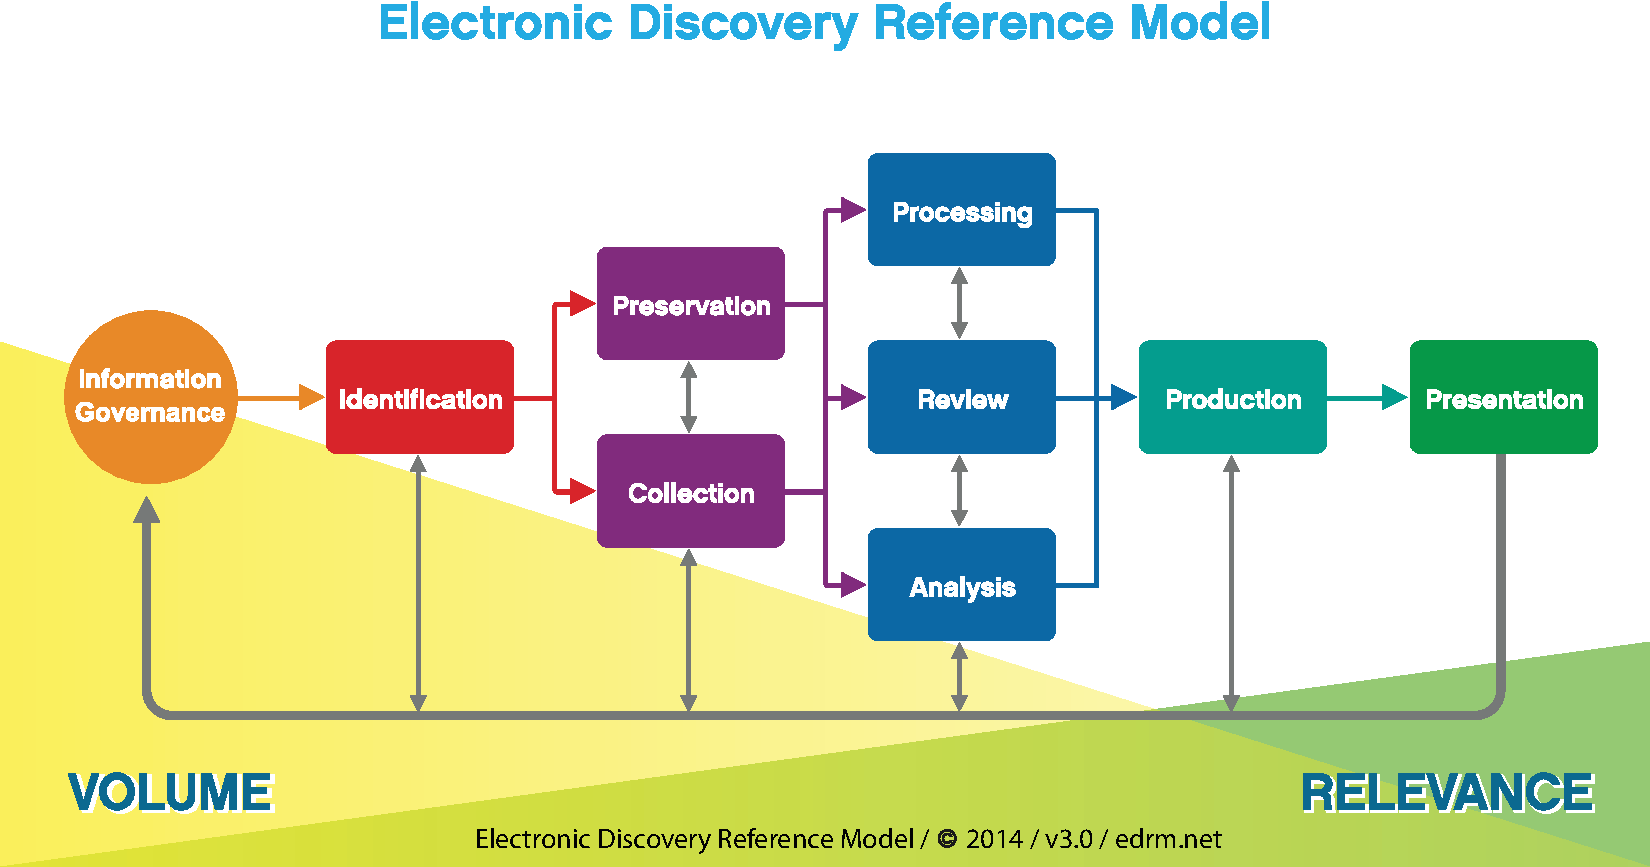
\includegraphics[width=0.7\linewidth]{./fig/EDRM-Chart_v3}
%   \caption{The Electronic Data Reference Model.}
%   \label{fig:edrm}
% \end{figure*}


\section{Motivation}
Over the past decade the use of data mining principles in software engineering has increased sharply. Examples include mining software repositories and data guided software analytics. In this work we aim to explore the relevance of lessons learned from software engineering practices when applied to better industrial data mining. To highlight this, we use the e-discovery process at LexisNexis as a case study. E-Discovery generally refers to the process by which electronically stored information pertinent to some matter, which in our context is the subject of a civil litigation, is extracted. This being an emerging field, it is our belief that lessons learned from decades of software engineering research can be leveraged to improve this process.

\subsection{E-Discovery at LexisNexis}
\label{sect:edisc}
The chief venue for E-discovery is in civil litigation whereby one party (the producing party), in possession of materials which are pertinent to legal case, makes available to the other (requesting party). Upon reception of a request, it is the duty of the producing party to make an inquiry to find all reasonably relevant materials in their possession and turn them over to the requesting party.
             
Initially, this review process was conducted by a group of attorneys. They read through all the documents one at a time and marking them as important or otherwise with tags based on the document's responsiveness to the request. This method of search is now known as \textit{linear review}. The rate of review depended on several factors collection, requests, and reviewers. The typical review rate was a few minutes per document~\cite{}. As is to be expected, with the growth in size of the collection, such a review process becomes more and more insupportable. To remedy this issue a higher degree of automation is to be adopted and these methods are now referred to as \textit{technology-assisted review (TAR)}.
%
The complex and nuanced process of e-discovery is summarized rather elegantly by a widely cited process model, known as the EDRM Reference Model. This model encompasses all the steps involved in an e-discovery process. Starting from "Information management" at the left, where the intent is to incorporate all the information processing that is required by the organization before the e-discovery process starts, to "Presentation" on the right, which involves the production of the discovered materials to support a legal analysis.

Our perspective in much narrower than that of the EDRM model, the principal focus of this paper is the fourth stage of this process. This stage comprises of three functions: Processing, Review, and Analysis. In the context of Technology-assisted Review, these functions can be interpreted as follows:
\bi
    \item \textit{Processing: } Involves feature generation and indexing of the available data set.
    \item \textit{Review: } Involves specification of sample documents with some human expertise in order to train the classifiers to perform automated classification.
    \item \textit{Analysis: } A form of formative assessment to evaluate the responsiveness of the classifier.
\ei

At the outset, TAR might seem to be a relatively straight forward task considering the advances in natural language processing and the number of machine learning tools at the disposal of the practitioner. However, the sheer number to available methodologies also makes it difficult to choose the right set of tools. 

The adversarial nature of litigation necessitates the need for rigorous validation of the obtained results in order to provide some assurance that software developed performs to the specified level of confidence and within its designed parameters and defined requirements. Undertaking such validation requires a closer understanding of the problem. 

\subsection{Your goals are not my goals}
The goals of e-discovery are unique and unlike several other classification problems in information retrieval. For instance, the problem of determining whether some document is responsive to a request is a binary classification problem for the simple reason that in the end, the document must either be determined to be responsive (and thus to be considered for production) or not to be responsive. 

Binary classification tasks are rather straight forward. However, upon reflecting on the nature of the problem being addressed, it is clear that E-discovery applications presents practitioners with some unique challenges: 
\be
\item  E-discovery emphasizes on absolute result sets instead of the conventional ranked retrieval; 
\item  In contrast to the high-precision focus of many end-user applications, such as Web search, e-discovery places great emphasis on achieving equally high recall.
\item  In addition to relative effectiveness of the the e-discovery process, evaluation strategies also stress on the absolute effectiveness. 
\item  E-discovery is a confluence of information retrieval and techniques from other fields (for instance, software engineering, computer forensics and document management); 
\ee

Indeed these challenges are not unique to e-discovery, neither are the proposed solutions. It is therefore critical to understand the goals and explore solutions accordingly.

\subsection{Stack Exchange}
Collections of Enron e-mails are perfect candidates for e-discovery process, they have been extensively used by e-discovery firms for several years~\cite{oard2013}. However, there doesn't seem to be a ``single'' Enron e-mail collection. As a result most results are not reproducible or comparable. We have therefore resorted to using the threads from various StackExchange sites\footnote{https://archive.org/details/stackexchange} for our experiments. The nature of StackExchange threads to mimic the unstructured textual nature e-mail threads was found to be very beneficial. The use of threads as units of retrieval has been reported in~\cite{elsayed08}.

Much focus on mining stack exchange data has been on multiclass tag prediction within stack exchange sites. However, the e-discovery at LexisNexis as described in \tion{edisc} is best modeled as a binary classification task. This requires that the stack exchange threads be processed accordingly. 

\subsection{Your data is not my data}
\label{sect:ydinmd}
The task of assessing a large collection electronically stored data is an expensive endeavor. Therefore it would be beneficial to be able to measure the performance of several systems on a common benchmark data set. In addition to this, it is crucial that we be able to replicate results obtained previously as closely as possible. An effective e-discovery collection is characterized by three core components -- reusability, comparability, and reproducibility. The test collection is tagged with descriptors to help identify the relevance of the documents retrieved from the collection. 

\begin{figure}[pbt]
    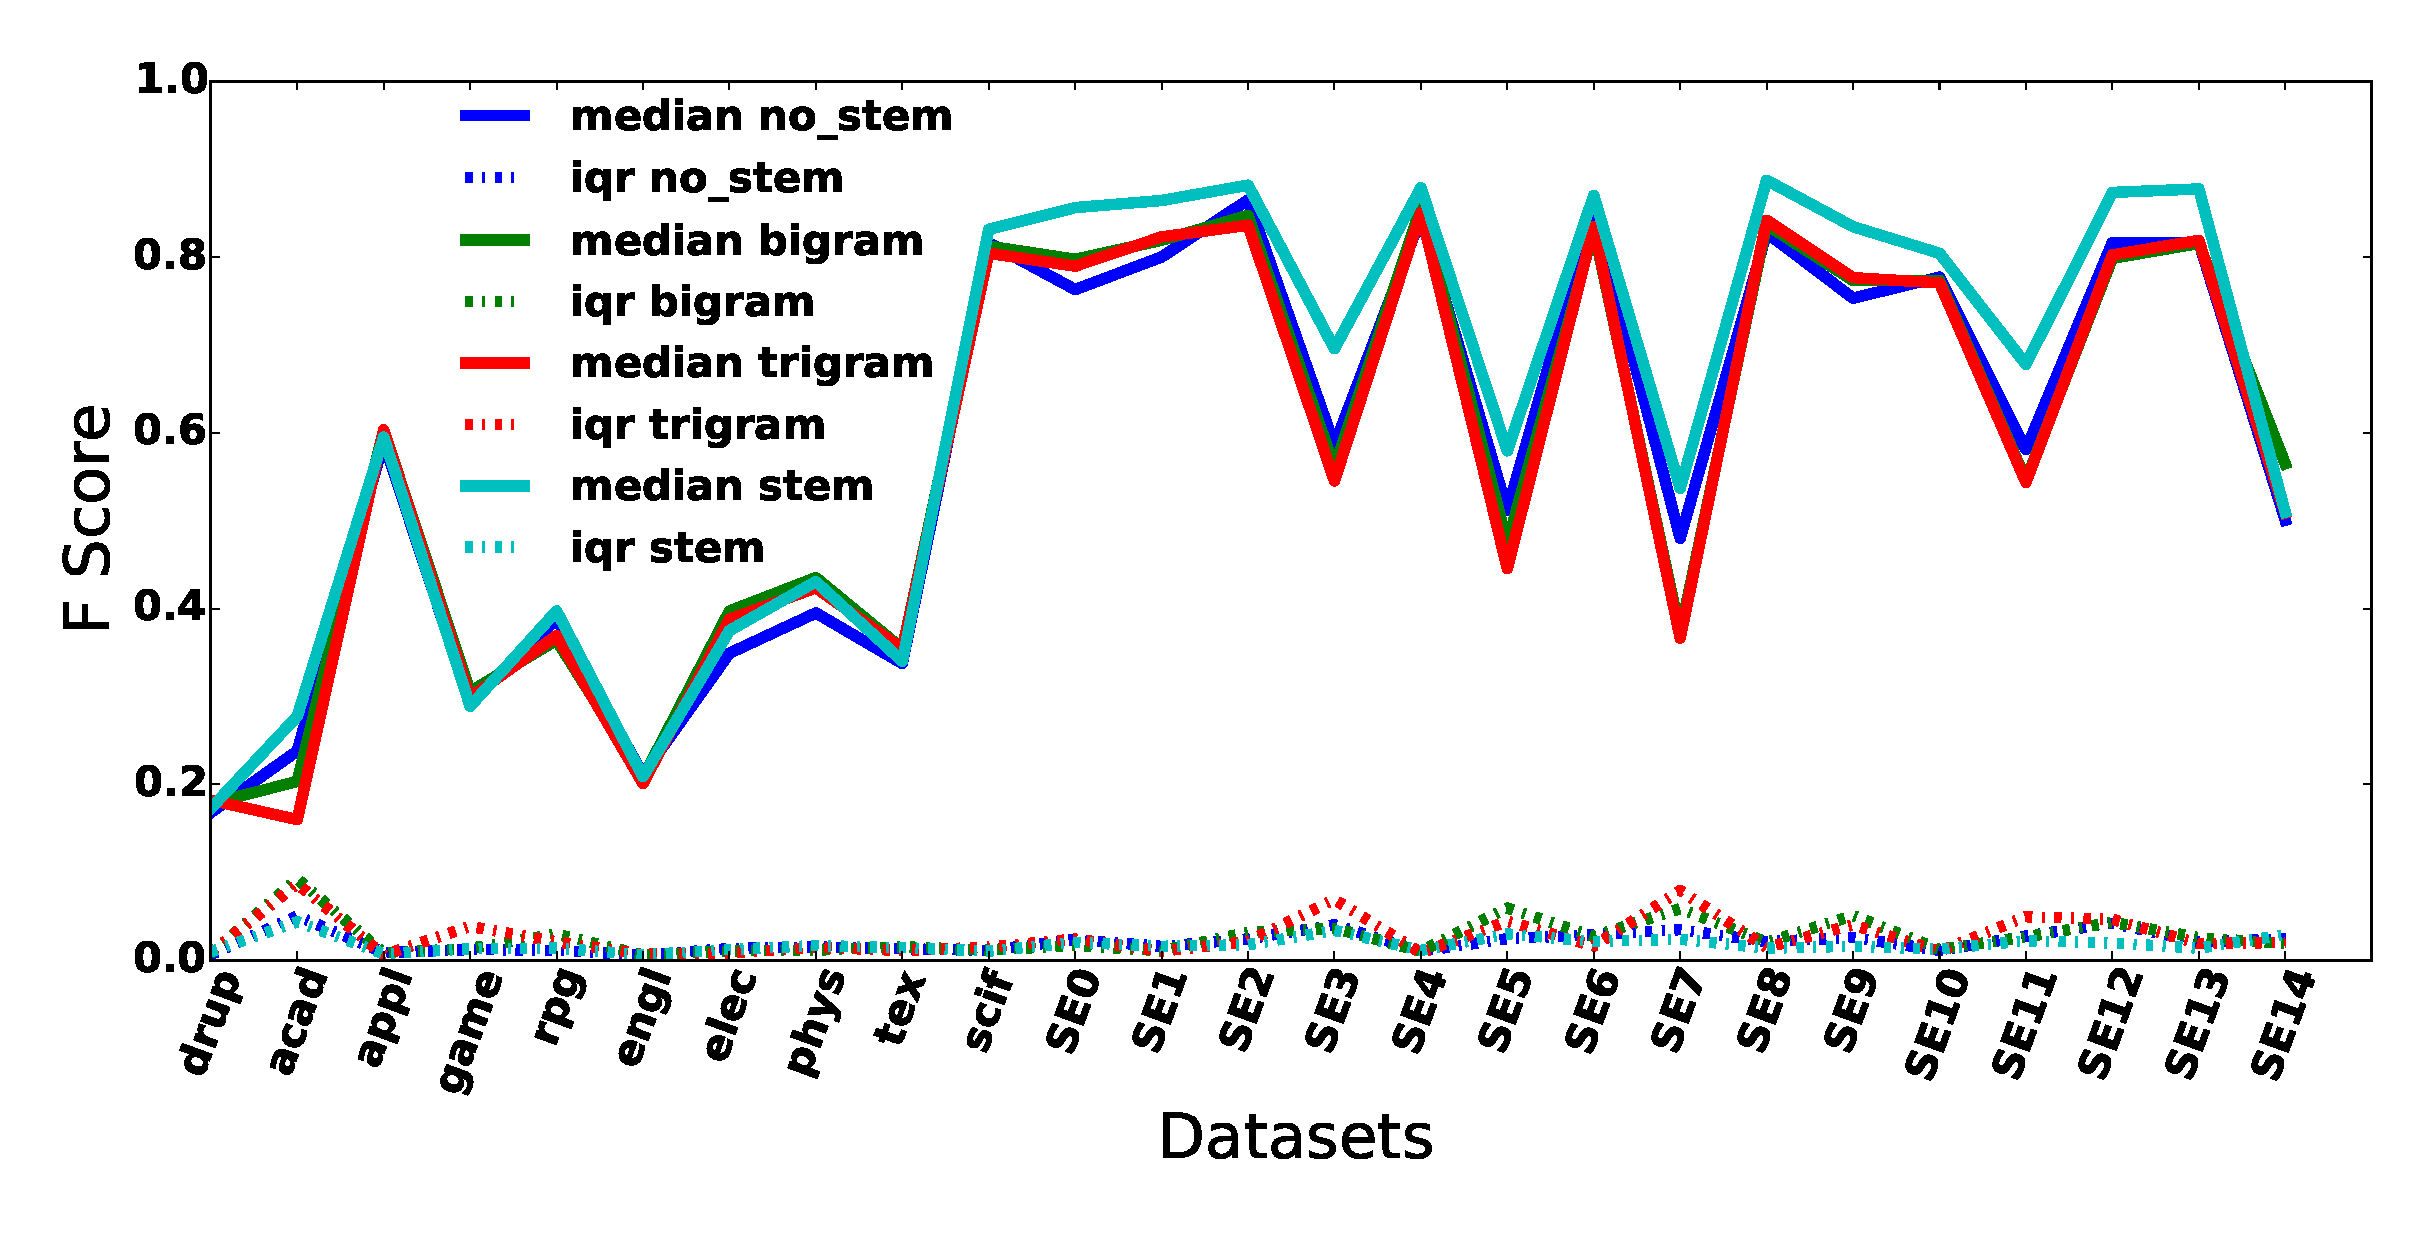
\includegraphics[width=0.99\linewidth]{./fig/pre.eps}
    \caption{Class distribution}
    \label{fig:token}
\end{figure}

There is ample literature on creation of test collection and information retrieval~\cite{sanderson2010test}. However, our focus here is on matters pertaining to e-discovery. There are notable differences between e-discovery and other information retrieval tasks, chief among these is the need for a different approach to selecting which documents should be judged for relevance. This process still required some amount of human intelligence, according to Baron et al.~\cite{baron2006trec} the report review rates for different topics at the TREC 2006 Legal Track ranged from 12.3 to 67.5 documents per hour, and averaging 24.7. In 2007, the average review rate was around 20 documents per hour, and around 21.5 per hour in 2008~\cite{oard08}. Roitblat et al.~\cite{roitblat} reported that for a large-scale review, 225 attorneys were required to each work nearly 2,000 hours to review 1.6 million documents, at a rate of 14.8 documents per hour. Borden~\cite{borden} cites a review of ``fairly technical'' documents running at the rate of 45 documents per hour, and states 50 to 60 documents per hour as the ``e-discovery industry average.'' It is therefore obvious that as the collection size increases it is not practical to assess every document for it relevance. Besides the arduous task of assessing millions of documents, it is also not a cost effective process, our industrial partners at LexisNexis report that attorneys are paid \$5 for every document they review. As a result, in e-discovery practitioners usually work with a very small subset of the original collection. Even though the number of documents in the collection is large, the TAR process uses only a small subset of labeled documents for training. In addition to this, the prevalence of responsive documents in a corpus is extremely low. It ranges from 2\% to 5\%. 

It is therefore necessary to negotiate an exemplary data set from the client prior to the start of the project. Such representative collection is very useful to understand the right options to explore. To understand the importance of this consider Figure~\ref{fig:token} which shows the impact of tokenization on several data sets. The image contains results on 2 groups of data sets, the first half contains results of tag prediction within sites where as the second half of the data sets show site prediction. Notice how even for simple preprocessing techniques like tokeniztion there are vast differences between the two data sets.


\subsection{What can SE teach Big Data?}
% Over the past decade the use of data mining principles in software engineering has increased sharply. In this work we ask what lessons can be learned from software engineering practices to better industrial data mining in the form of e-discovery. The relevance of this question can be justified by looking at the market for vendors of e-discovery systems, et. al \cite{} estimate this at \$US 1 billion in 2010. Additionally, several times this figure is spent on the staffing and processing costs to use the systems effectively \cite{}[108]. From a software engineering perspective, effective usage of e-discovery depends on two goals: (1) Enhancing the effectiveness of the system for some level of human effort, thereby increasing the return on investment, and (2) Minimizing costs. Furthermore, these fundamental technologies developed for e-discovery may have applications in other fields as well. For example, the preparation of systematic reviews of recent research on specific topics in medicine might benefit from advances in high-recall search [67], and personal information management might benefit from advances in search technology that focus specifically on e-mail (which at present is of particular interest in operational e-discovery settings).
The relevance of Software engineering principles can be justified by looking at the market for vendors of e-discovery systems, et. al \cite{} estimate this at \$US 1 billion in 2010. Additionally, several times this figure is spent on the staffing and processing costs to use the systems effectively \cite{}. From a software engineering perspective, effective usage of e-discovery depends on two goals: (1) Enhancing the effectiveness of the system for some level of human effort, thereby increasing the return on investment, and (2) Minimizing costs. 

Brook's law: half the time spent in testing. It is not sufficient to use these data miners once, we need a validation rig. Systems stuff for validation purposes. Leveraging the power of HPC at NC State.

Further, these fundamental technologies developed for e- discovery may have applications in other fields as well. For example, the preparation of systematic reviews of recent research on specific topics in medicine might benefit from advances in high-recall search [67], and personal information management might benefit from advances in search technology that focus specifically on e-mail (which at present is of particular interest in operational e-discovery settings).


\section{Test Collection}

\begin{figure}[t]
  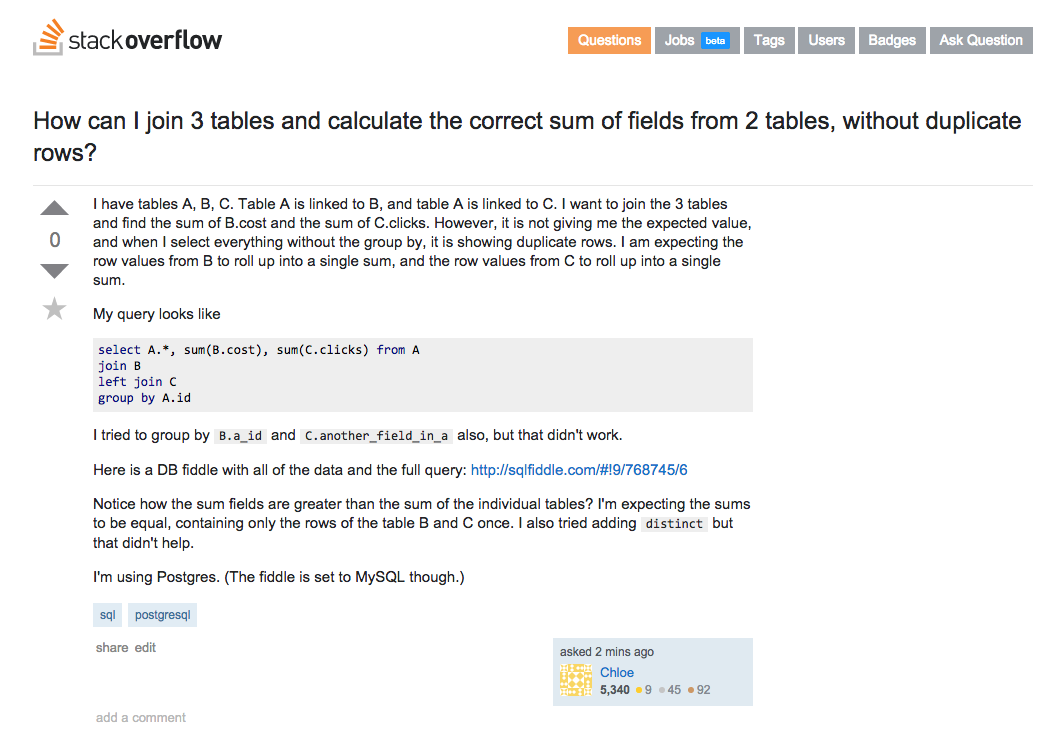
\includegraphics[width=\linewidth]{./fig/example.png}
  \caption{StackOverflow Post}
  \label{fig:example}
\end{figure}

Data for our experimentation is gathered from StackExchange sites. An example of StackOverflow post is shown in Figure \ref{fig:example}. We undertake classification at two levels of granularity: site level and tag level. Twenty data sets generated from StackOverflow posts are used in the experiments. Each data set contains ten thousand posts. The title and body of the posts are concatenated to form the independent variables for classification. The first tag for the posts are treated as the class of the post. Since many classes have such a small population, only the classes with top 19 population are kept while all the other classes are combined into one single class 'others'.

Literature can be found on tag-level predictions of StackExchange Data sets \cite{moharanatag,stanley2013predicting,kuo2011word}. The differences are that they have multi-classification tasks while ours is binary-classification, and they predict tags while we predict sites. Despite the differences, certain methods and structures help the construction of our experiments.

Moharana, 2013 \cite{moharanatag} has tried different approaches to predict StackOverflow tags. Three different classifiers, Linear SVM, Multinomial Naive Bayes, and Perceptron, with two different features, term frequency and tf-idf, are tested. The task is a multi-classification problem. The performance is measured by $F_{1}$ score. Best approach in \cite{moharanatag} is linear SVM + tf-idf and the $F_{1}$ score is $0.5358$.

Clayton and Byrne, 2013 \cite{stanley2013predicting} have worked on StackOverflow tag prediction and developed an ACT-R inspired Bayesian probabilistic model. This approach achieves a $65\%$ of accuracy by choosing the tag that has the highest log odds of being correct, given the tag's prior log odds of occurrence and adjusting for the log likelihood ratio of the words in the post being associated with the tag. The task is a multi-classification and multi-label problem.

Kuo, 2011 \cite{kuo2011word} has also worked on StackOverflow tag prediction. Kuo uses a co-occurrence model that predicts tags based on the relation (co-occurrence) between the words and tags. Initially built for next-word prediction in large documents, this model is adapted to the StackOverflow dataset by constraining the next word predicted to only tags. A $47\%$ classification accuracy is achieved.

Another model called SNIF-ACT (Fu \& Pirolli, 2007 \cite{fu2007snif}) also uses co-occurrences and can predict link traversal for search queries. The model predicts the most likely link that a person will click on by a search query (goal state) and fetched results. 

\section{Surprises}
\label{sect:Method}
Our validation strategy involved a greedy search in that space of the standard text mining practices. To our surprise, we discovered certain standard text mining practices are not always useful in some data sets. Listed below are some of our findings:
\be
\item \textbf{Tokenization:} Stemming and removal of stop words were generally useful. Bagging and shingling offered no noticeable benefits. 
\item \textbf{Featurization:} Contrary to popular recommendation, just using term frequency (TF) proved to work just as well as using TF-IDF.
\item \textbf{Normalization:} L2 normalization on rows was noticed be useful. No surprises hers, this adheres to the standard practice.
\item \textbf{Dimensionality Reduction:} Given how there is no difference between TF and TF-IDF, using hashing trick in place of TF offered an added benefit of using fewer dimensions.
\item \textbf{Data Balancing:} The low prevalence of "interesting" class in the test collection was handled remarkably well by SMOTE.
\item \textbf{Classification:} Although SVM is considered a superior classifier for text mining applications, it was surprising to note that Linear SVM outperformed other kernels.
\ee

\subsection{Performance Metrics}

%\textbf{RQ2} What is the proper performance metric for this task?

There are two contradictory goals that should be achieved according to our task: 

\textbf{a) Precision} ($p$) since all the documents being predicted as 'related' should be examined by human efforts, a high precision can greatly reduce the cost of this examination.

\textbf{b) Recall} ($r$) a high recall can reduce the number of 'related' documents that we failed to retrieve.

For the purpose of studying both precision and recall, we use:
 \mbox{$F_{1}=  2pr/(p+r)$}
as  our  performance metric.

\section{Experiments}
\label{sect:Experiment}



For each experiment, a 5 by 5 cross-validation ($20\%$ as training sample and $80\%$ as testing sample since in real tasks, the training sample is always less) is performed on 10 tag-level and 15 site-level data sets. The first ten data sets from left in Figure \ref{fig:all} are of tag-level while the last 15 are of site-level.



\begin{figure*}[t!]
    \centering
    \subfigure[Tokenization]
    {
        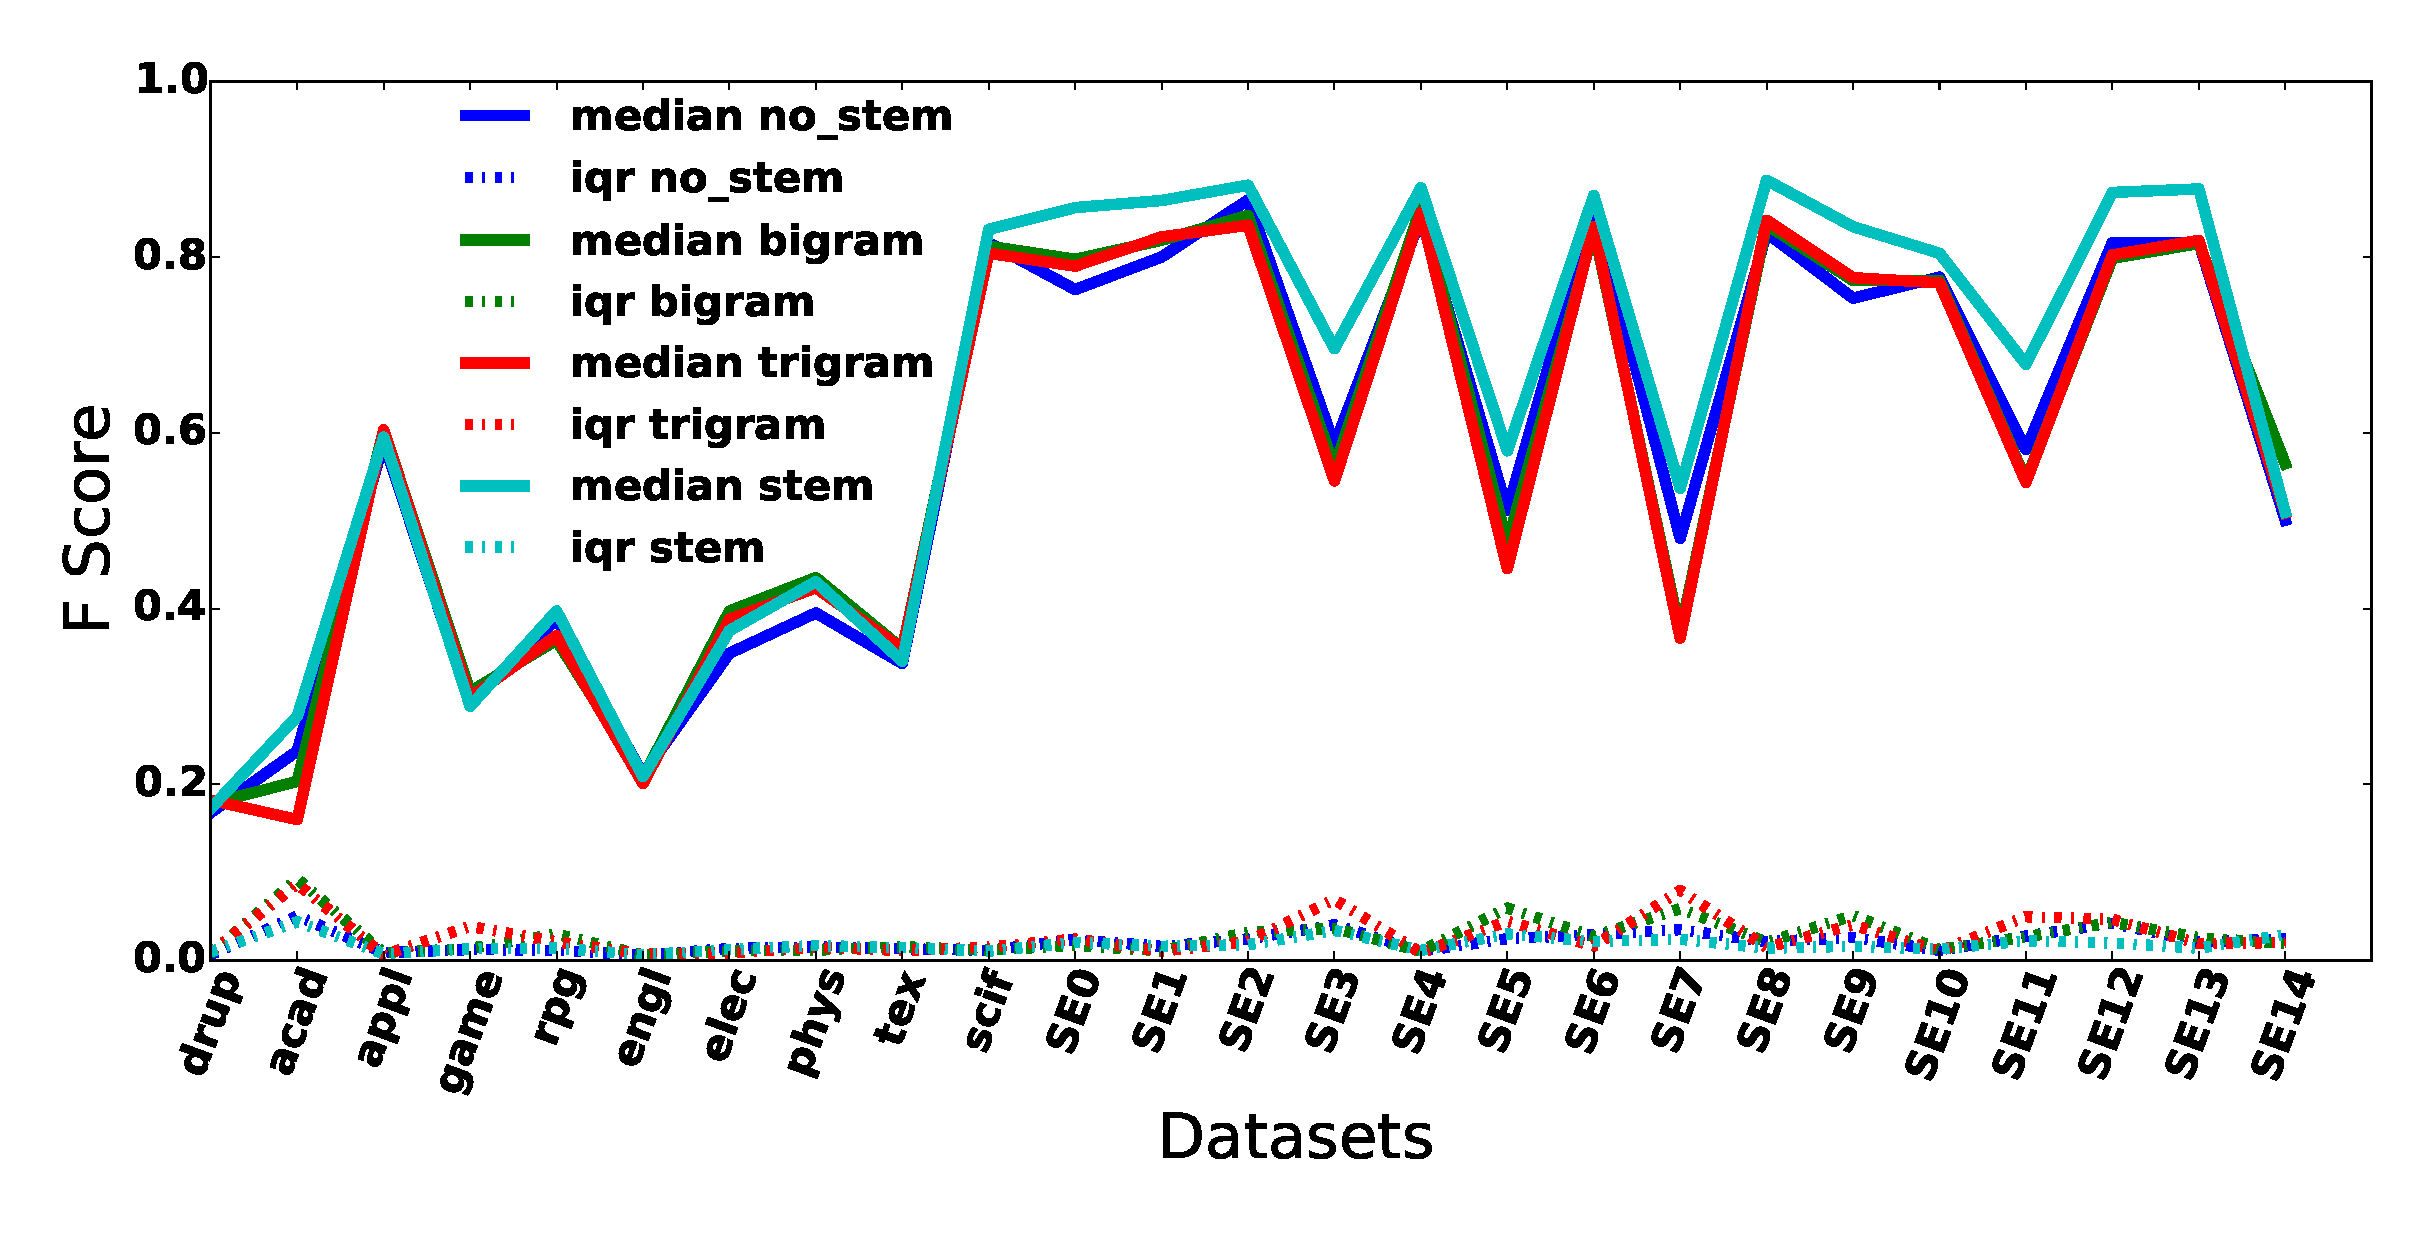
\includegraphics[width=0.48\linewidth]{./fig/pre.eps}
        \label{fig:pre}
    }
    \quad
    \subfigure[Featurization]
    {
        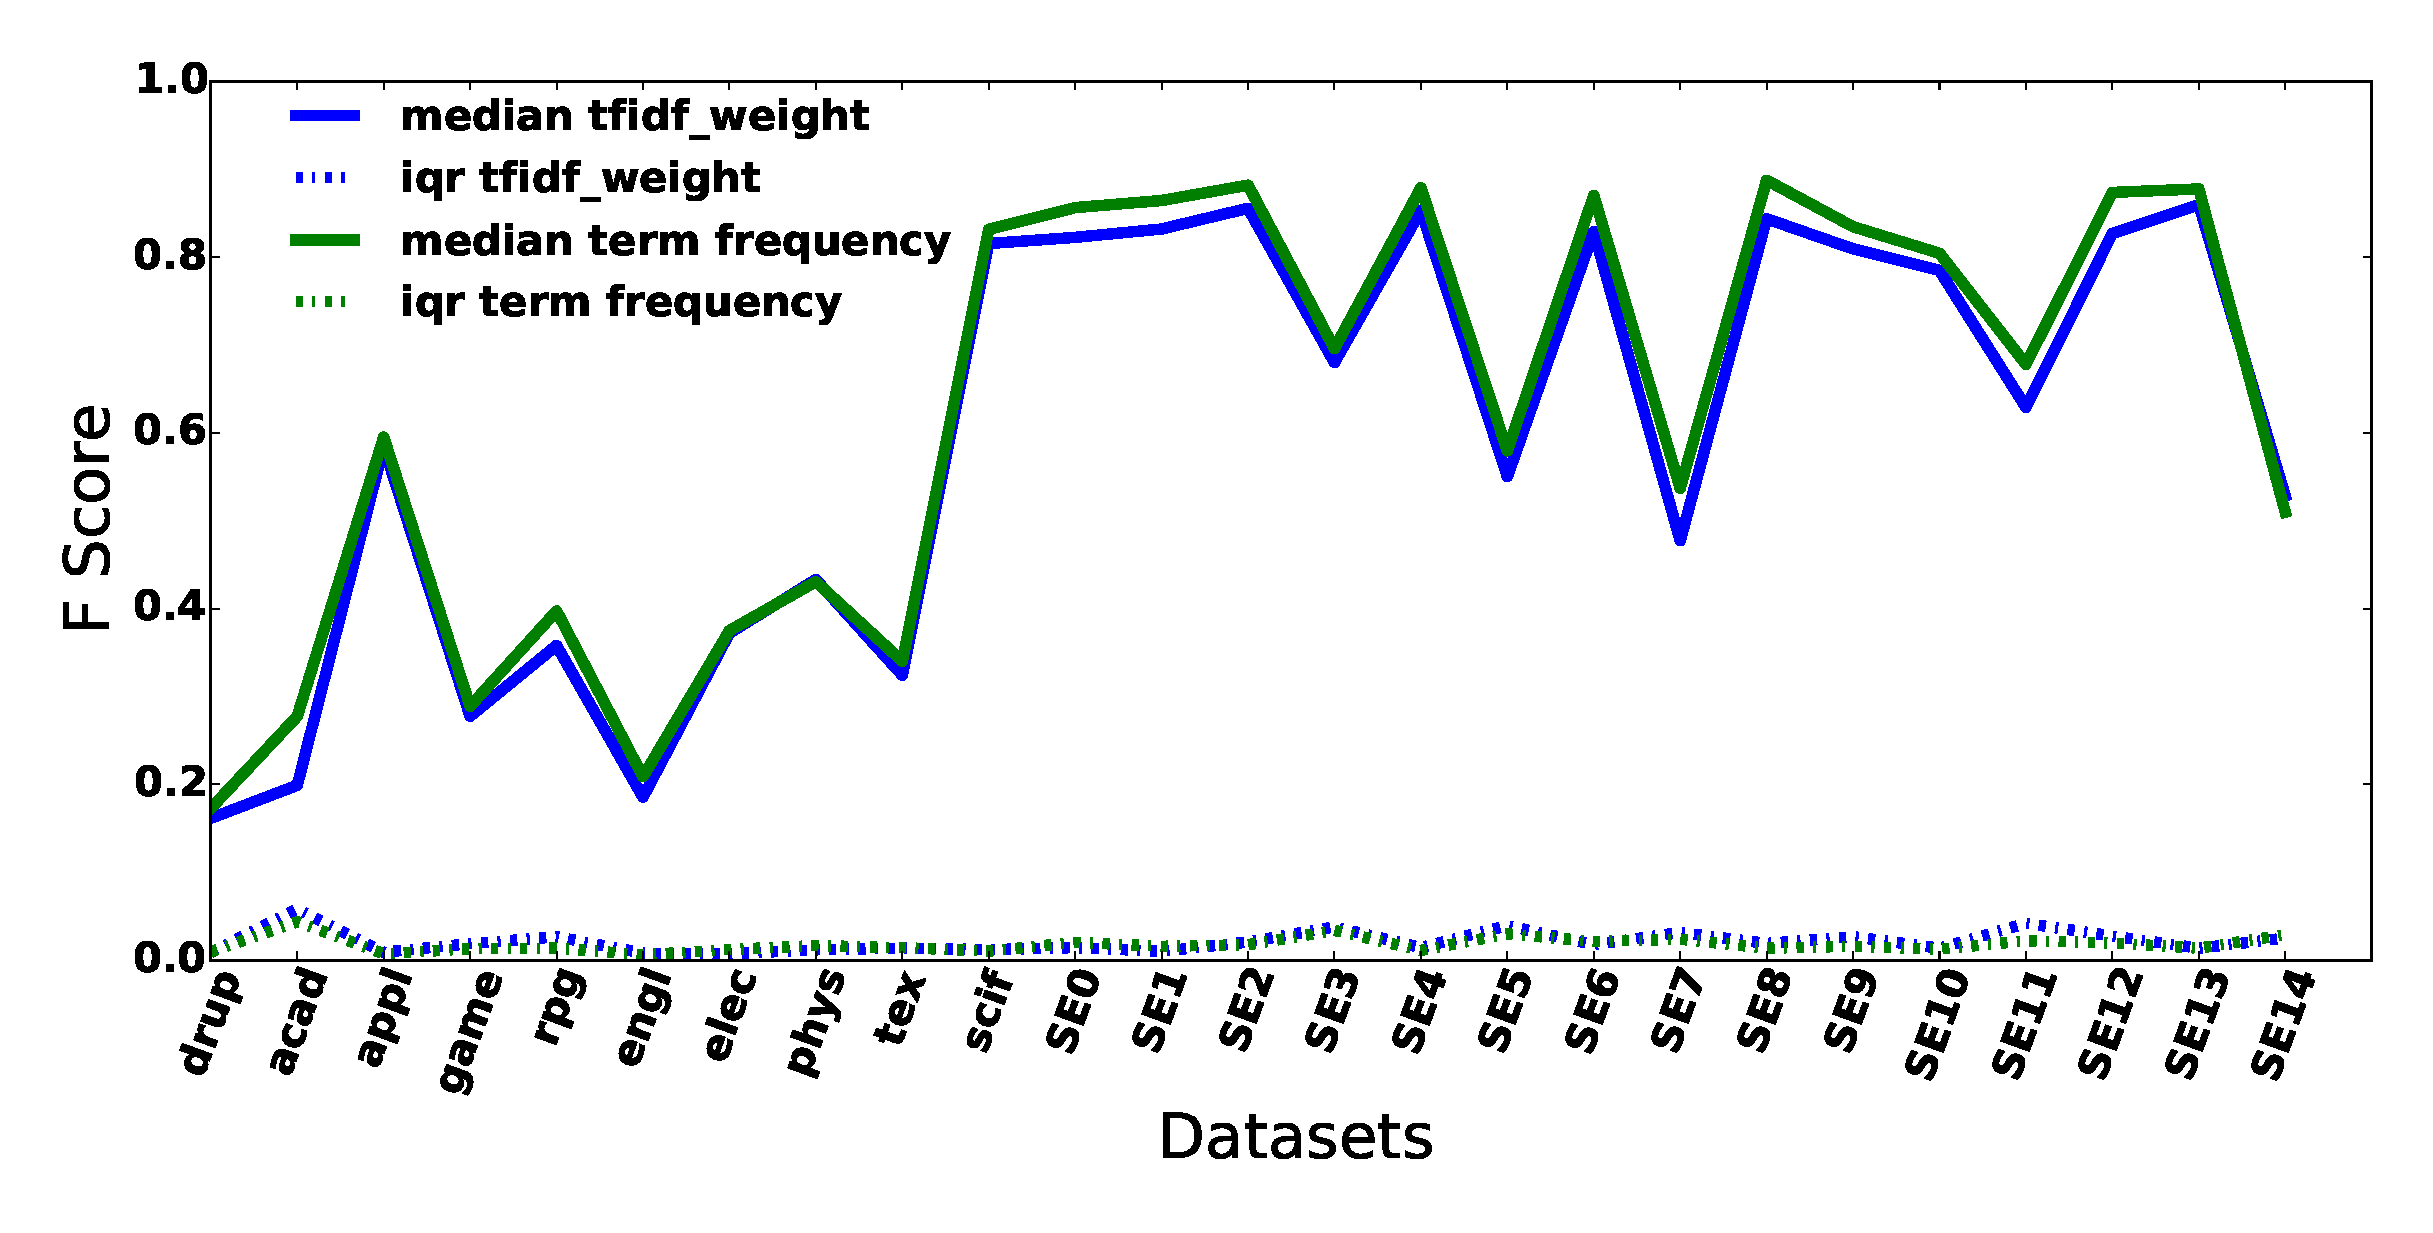
\includegraphics[width=0.48\linewidth]{./fig/fea.eps}
        \label{fig:fea}
    }
    \quad
    \subfigure[Dimensionality Reduction]
    {
        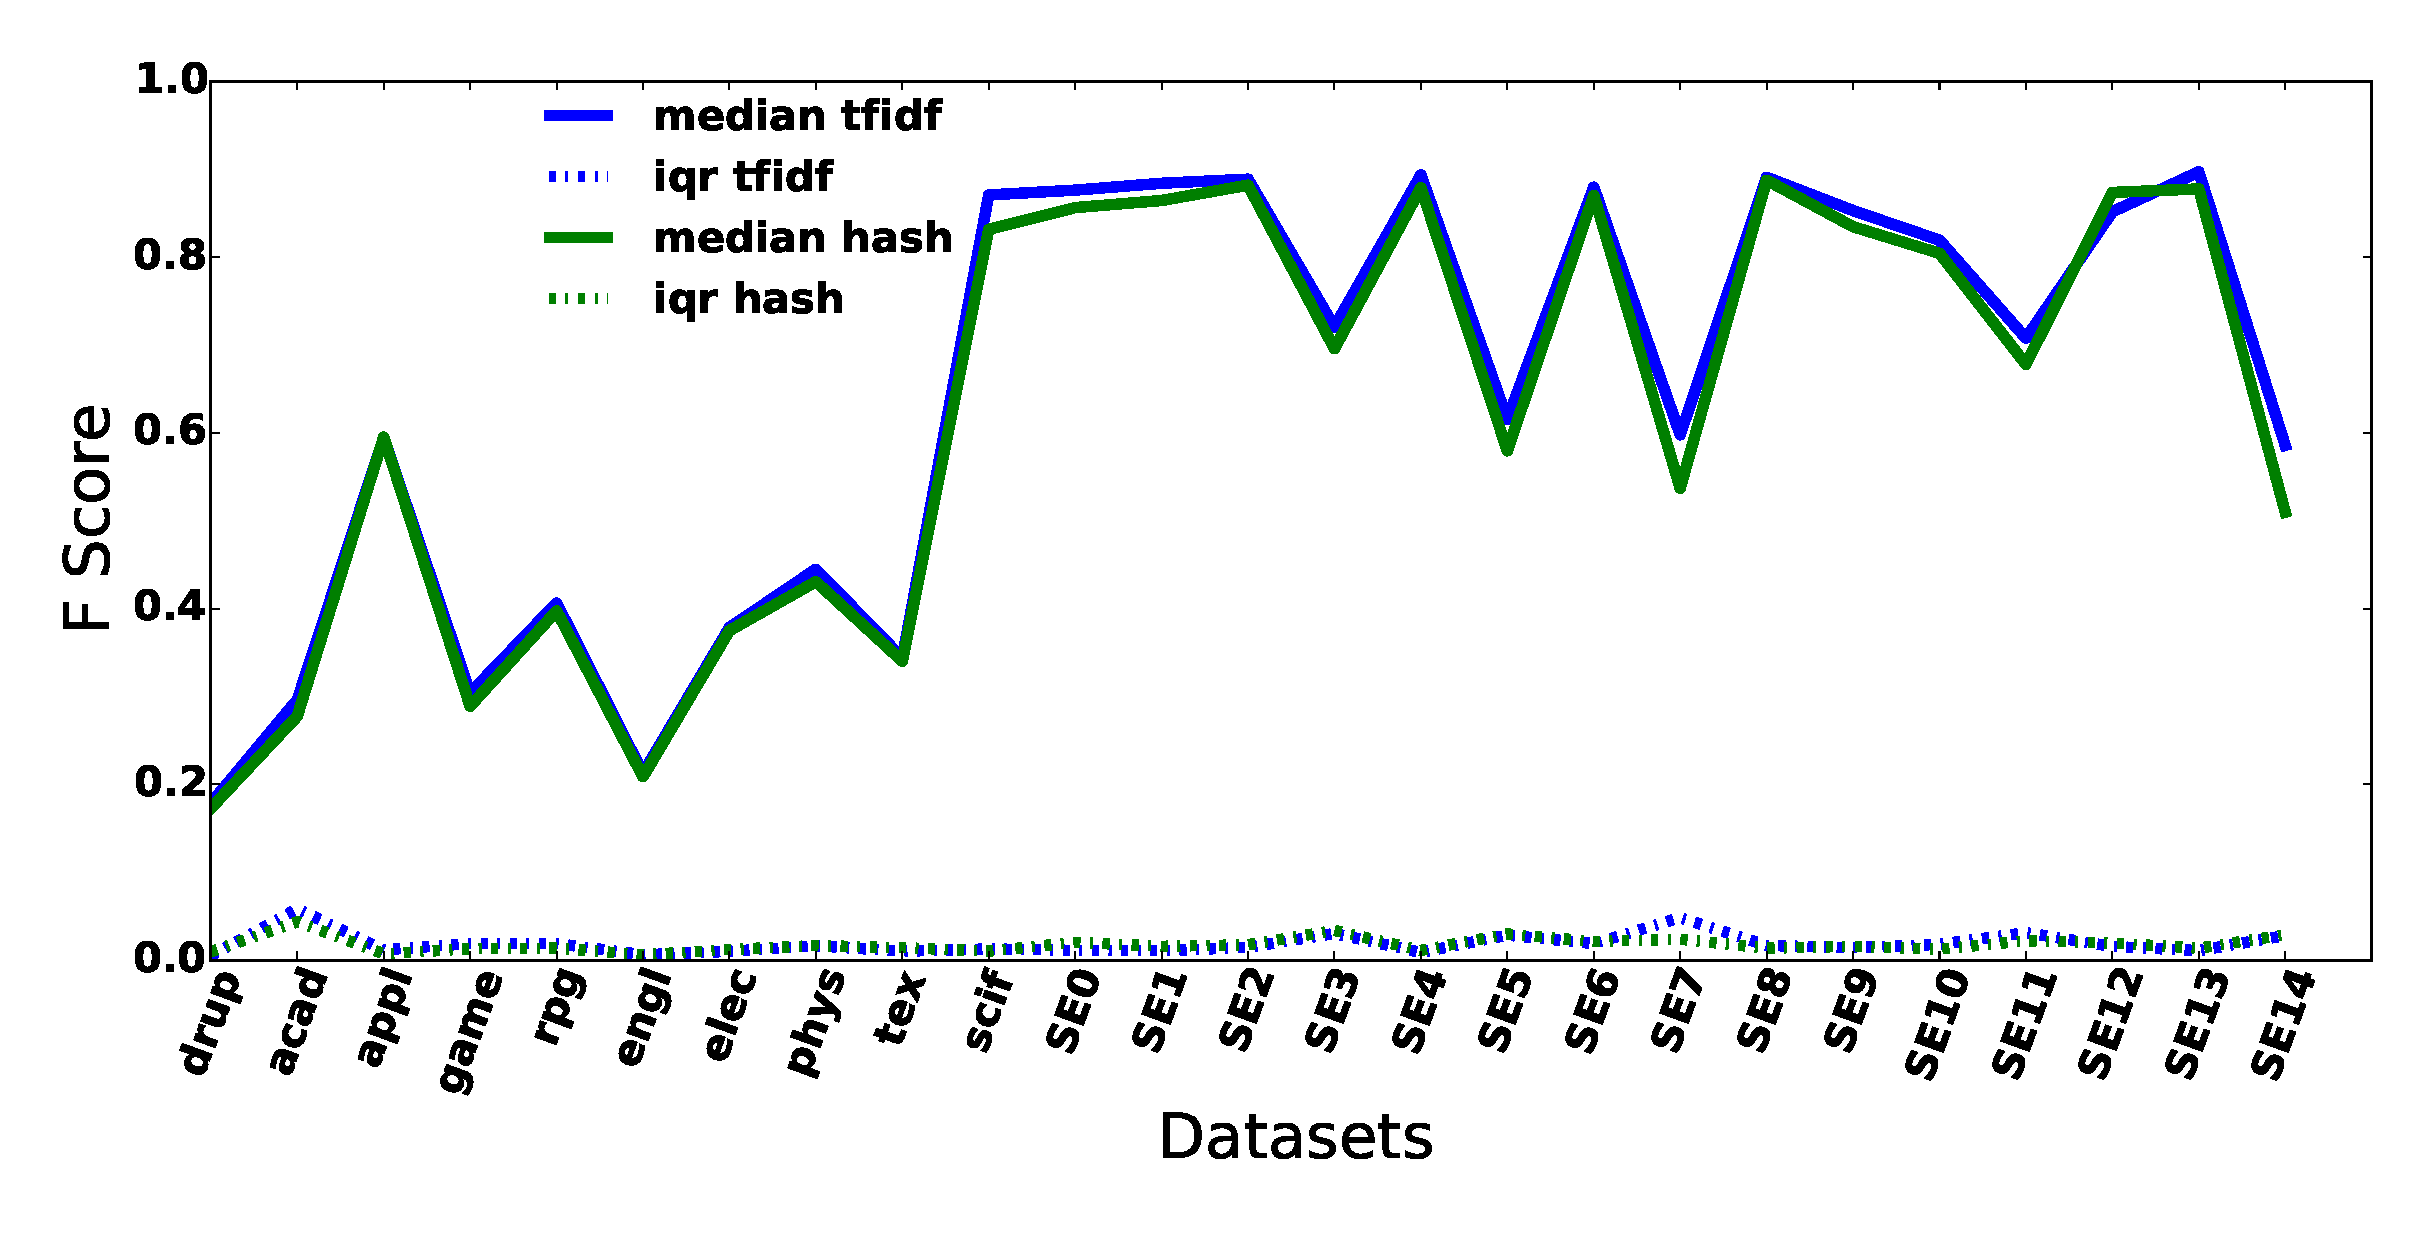
\includegraphics[width=0.48\linewidth]{./fig/sel.eps}
        \label{fig:sel}
    }
    \quad
    \subfigure[Number of Features]
    {
        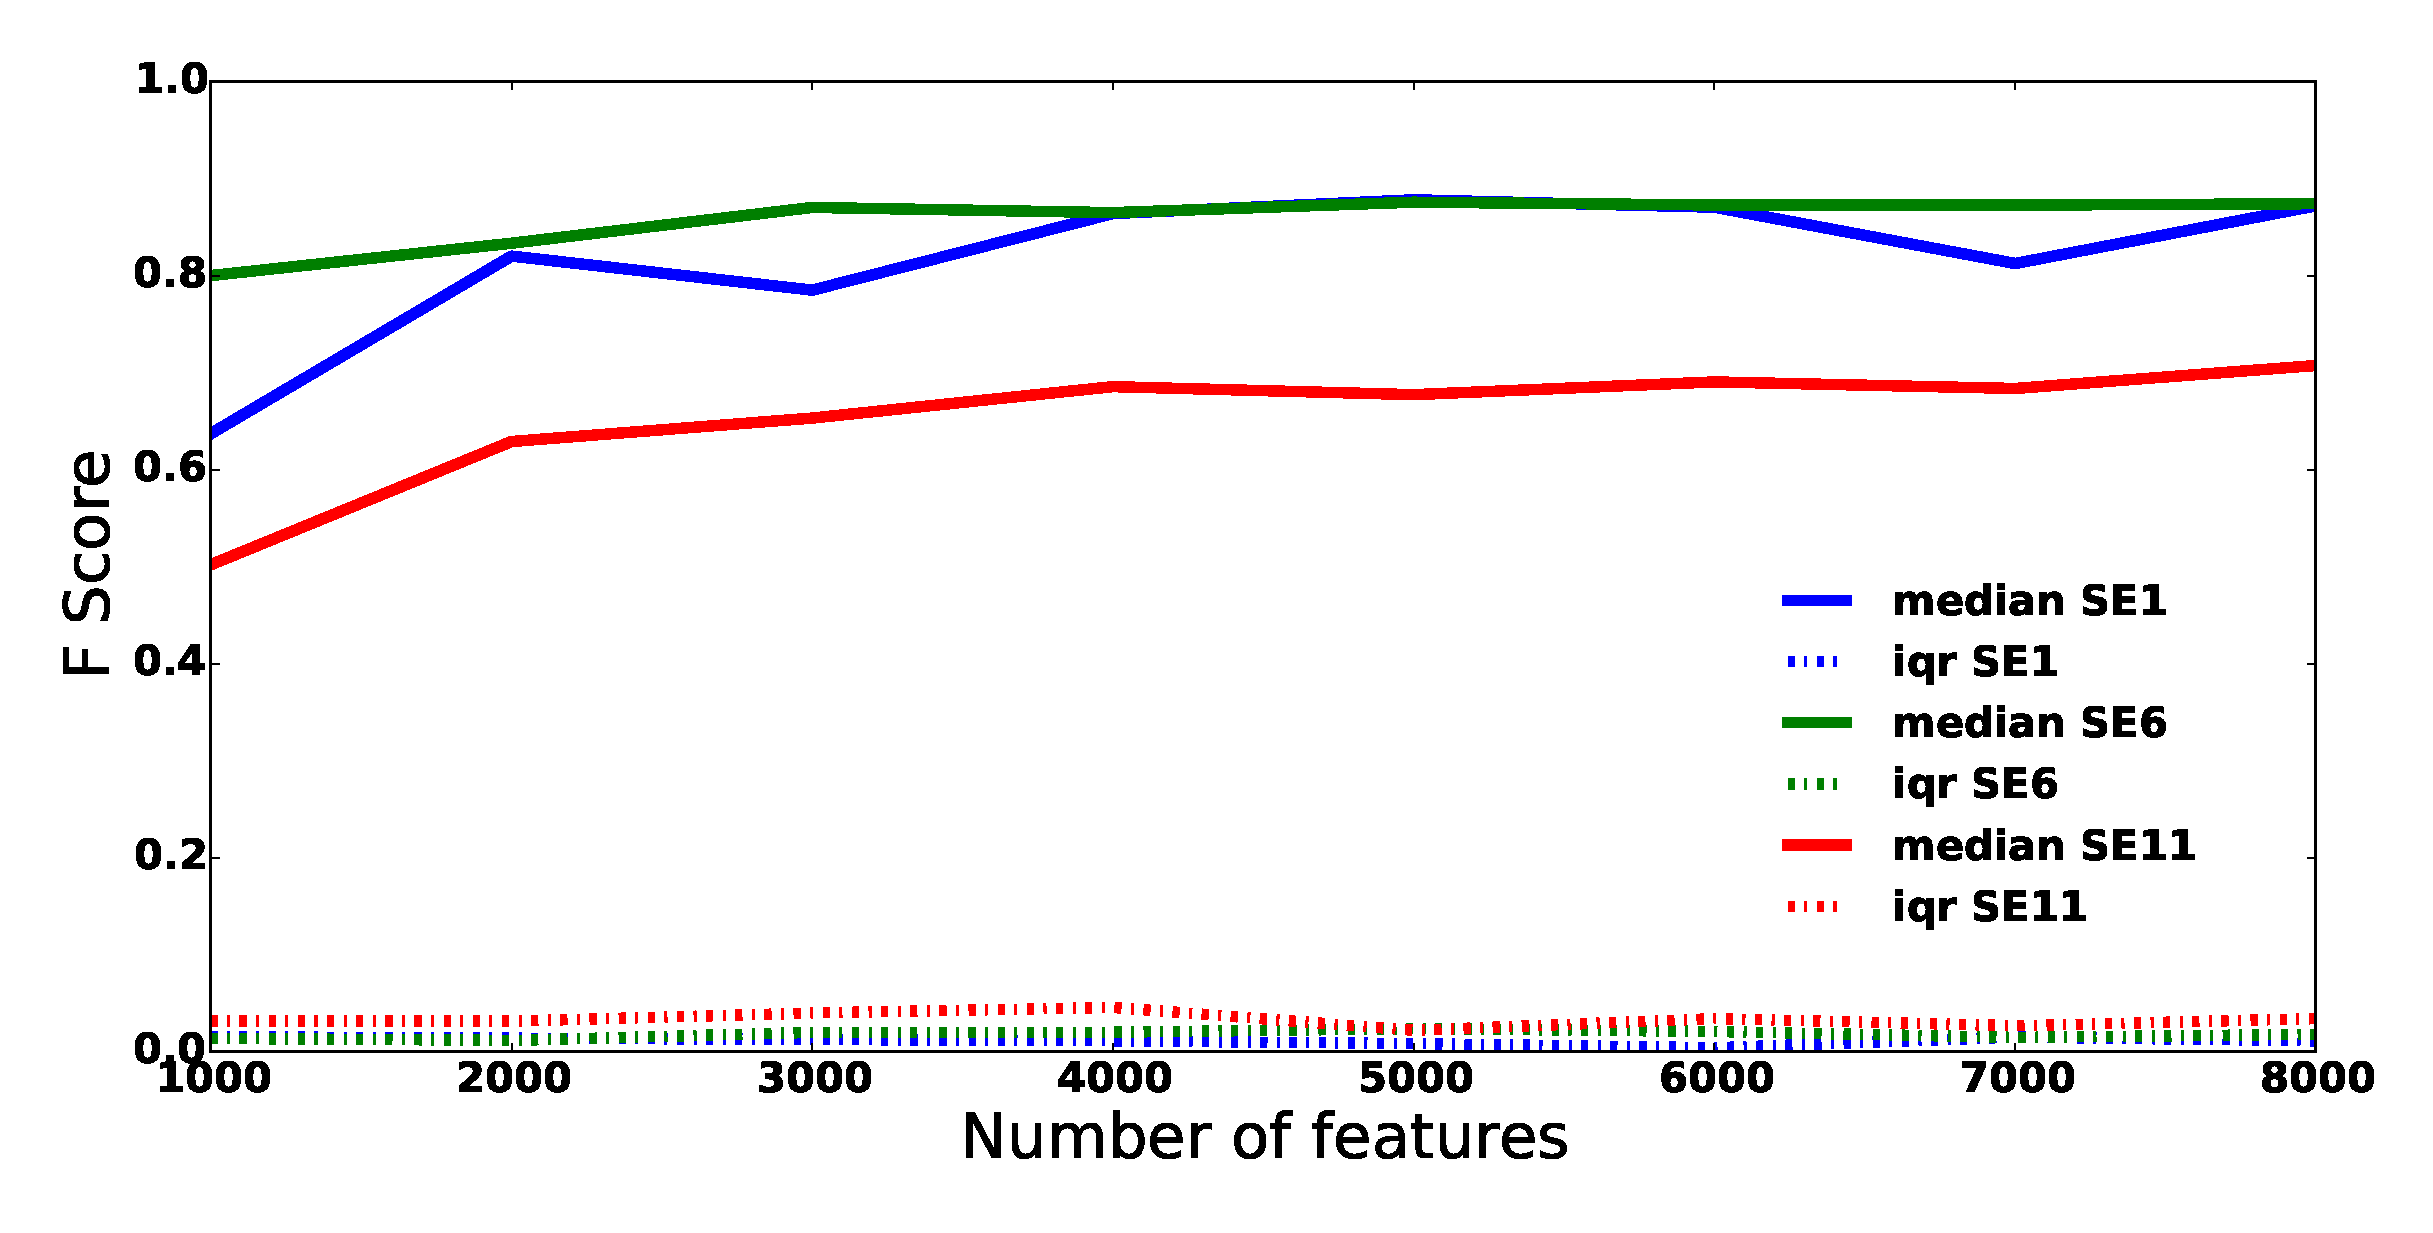
\includegraphics[width=0.48\linewidth]{./fig/fea_num.eps}
        \label{fig:fea_num}
    }
    \quad
    \subfigure[Normalization]
    {
        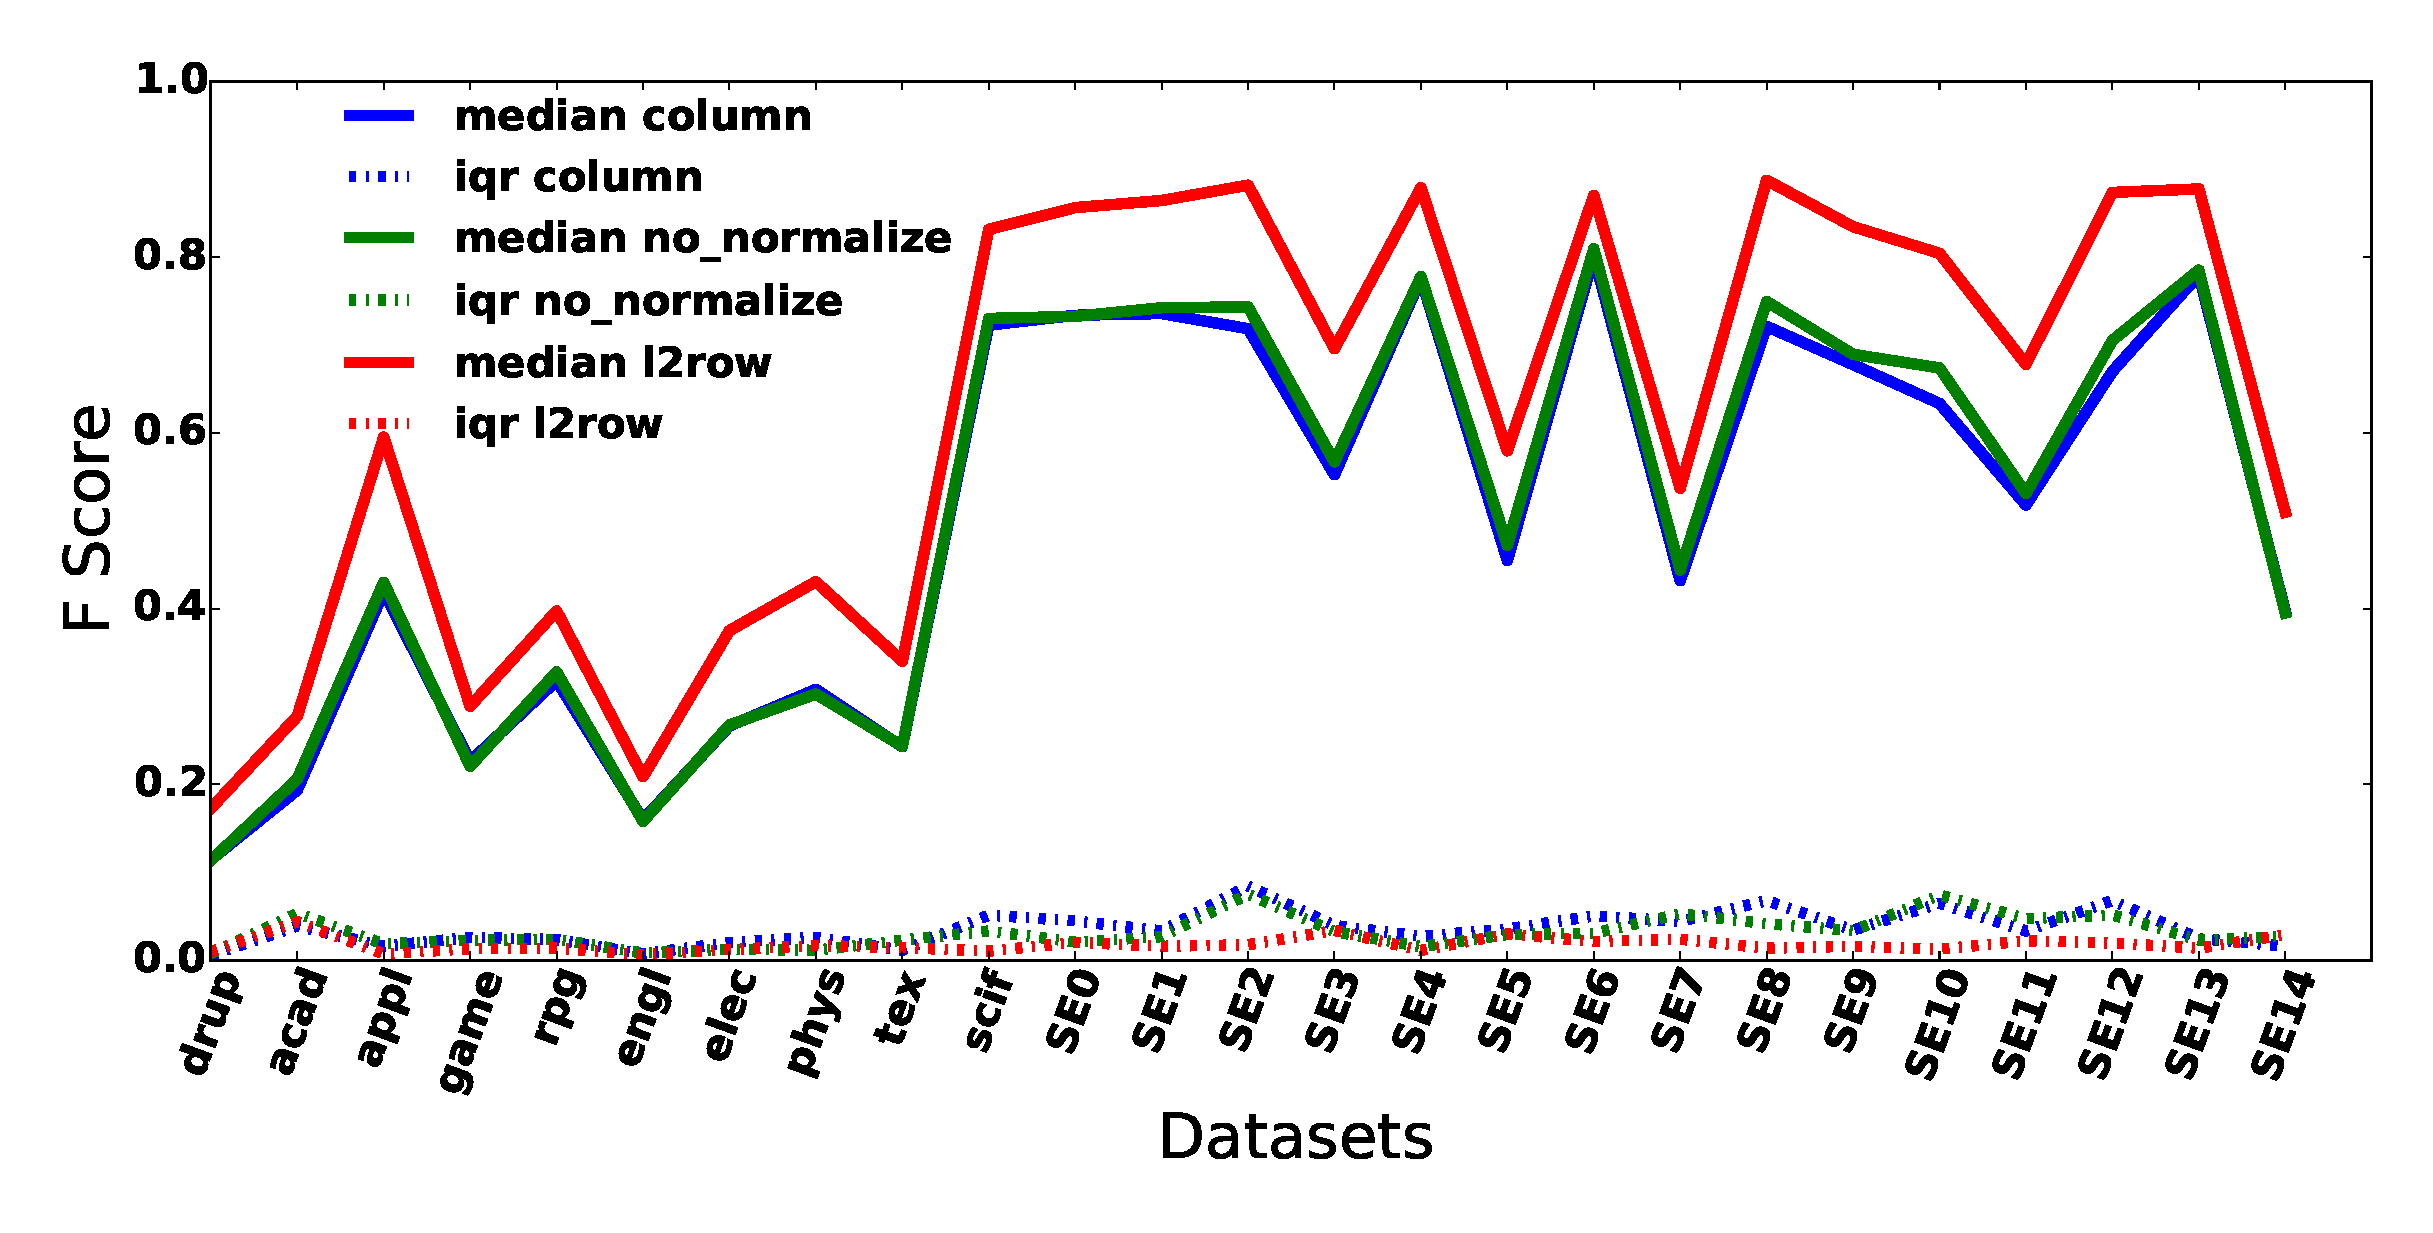
\includegraphics[width=0.48\linewidth]{./fig/norm.eps}
        \label{fig:norm}
    }
    \quad
    \subfigure[Data Balancing]
    {
        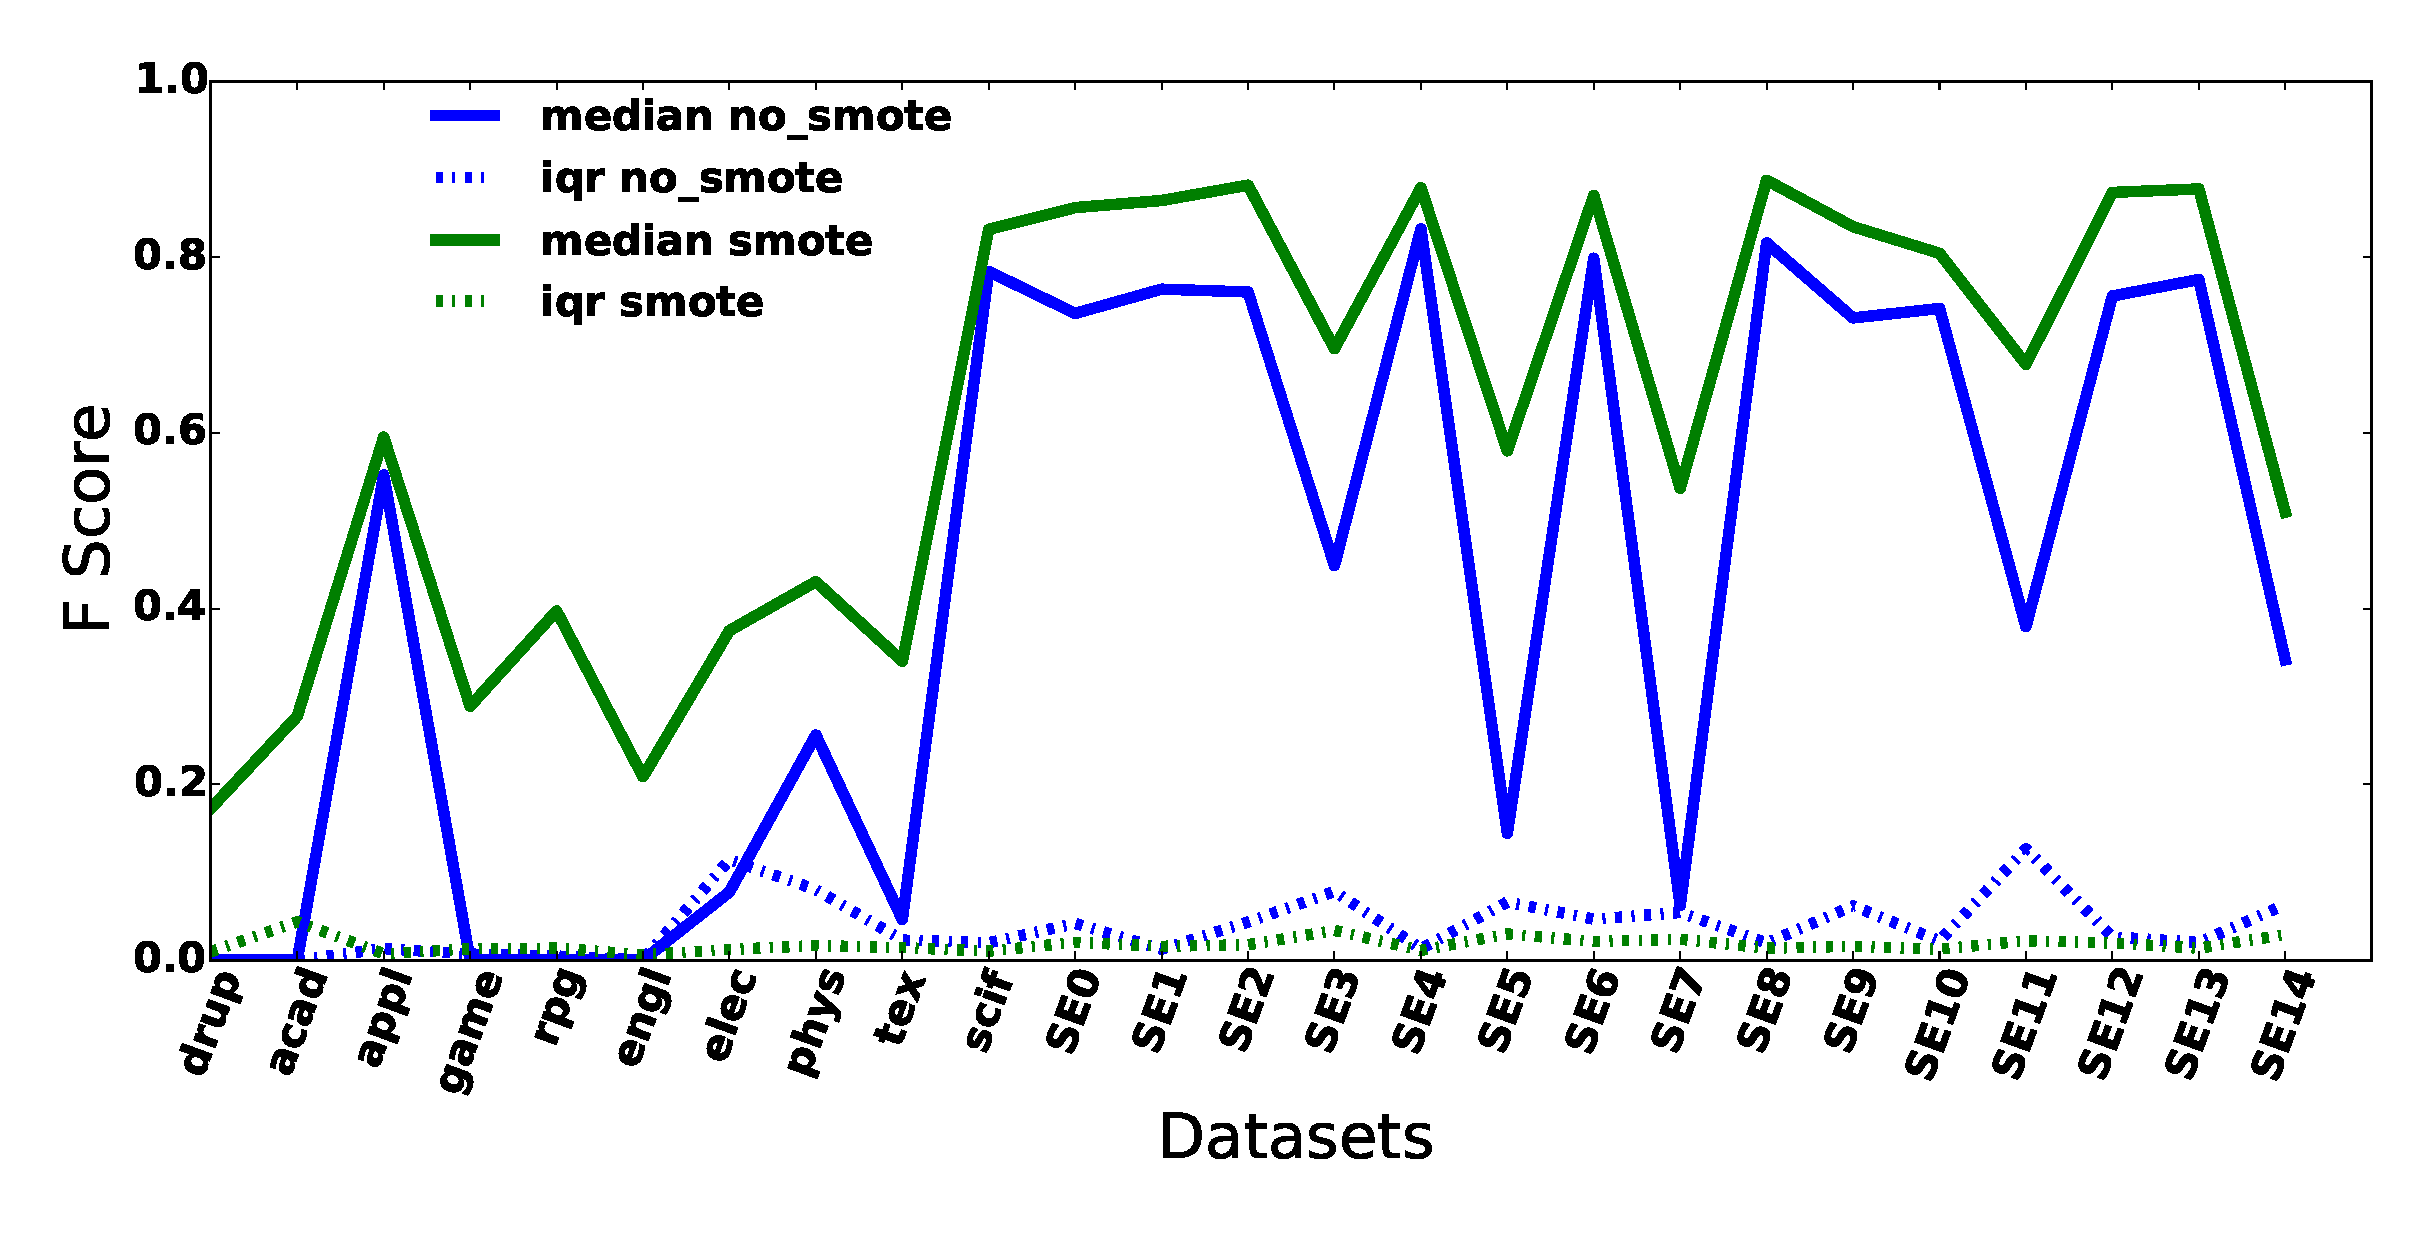
\includegraphics[width=0.48\linewidth]{./fig/balance.eps}
        \label{fig:balance}
    }
    \quad
    \subfigure[Classifiers]
    {
        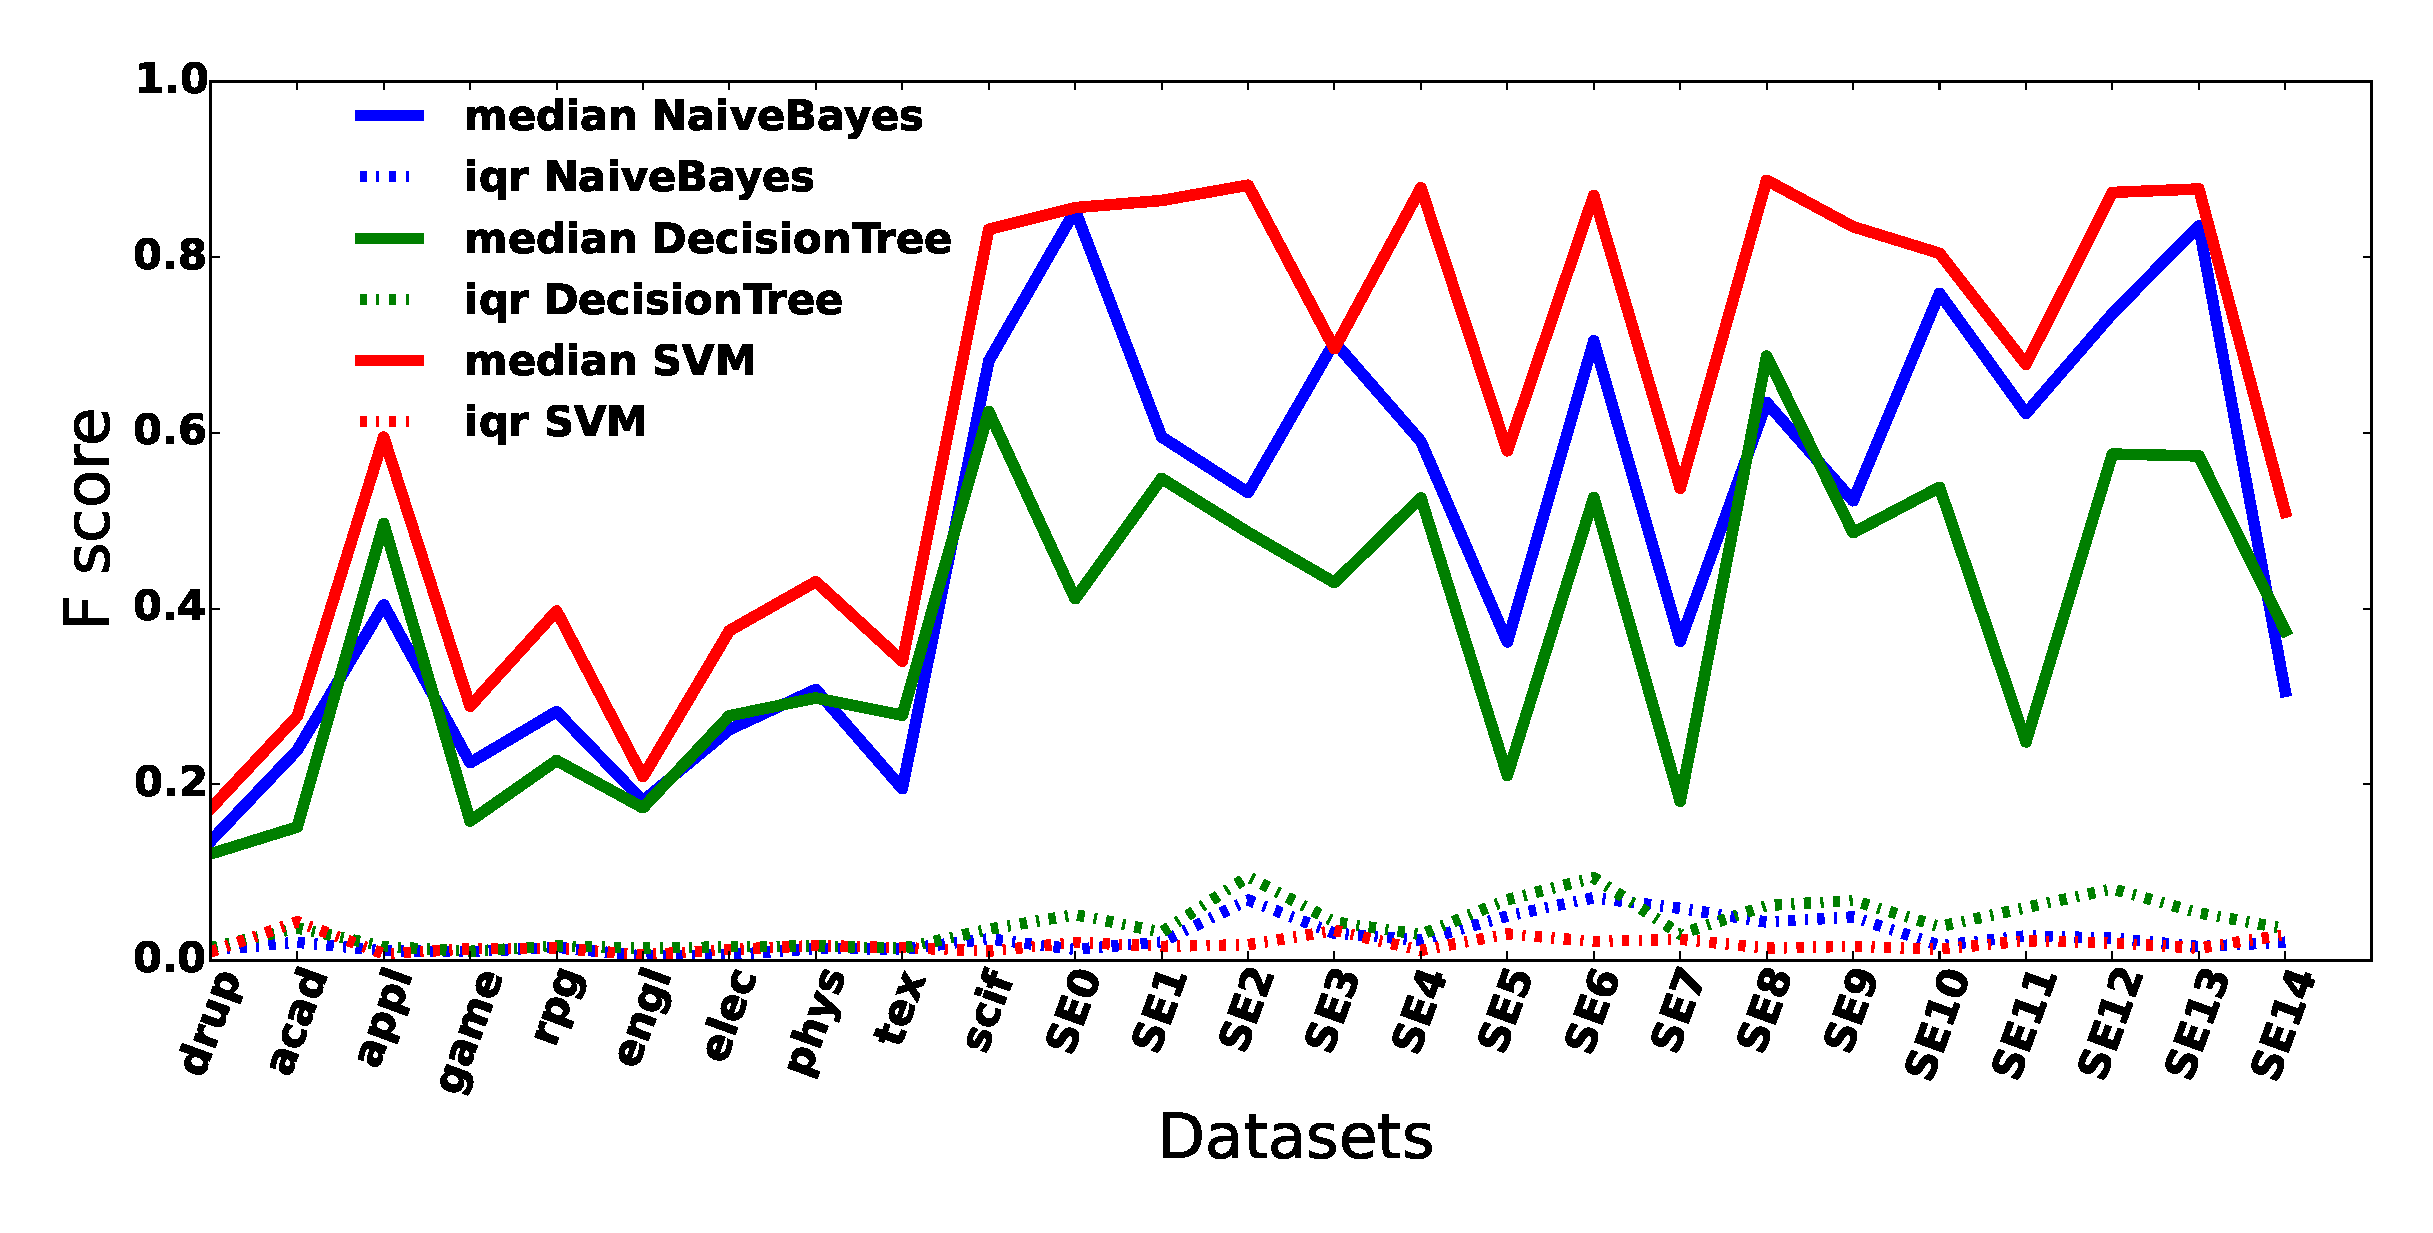
\includegraphics[width=0.48\linewidth]{./fig/algms1.eps}
        \label{fig:algms1}
    }
    \quad
    \subfigure[SVM Kernels]
    {
        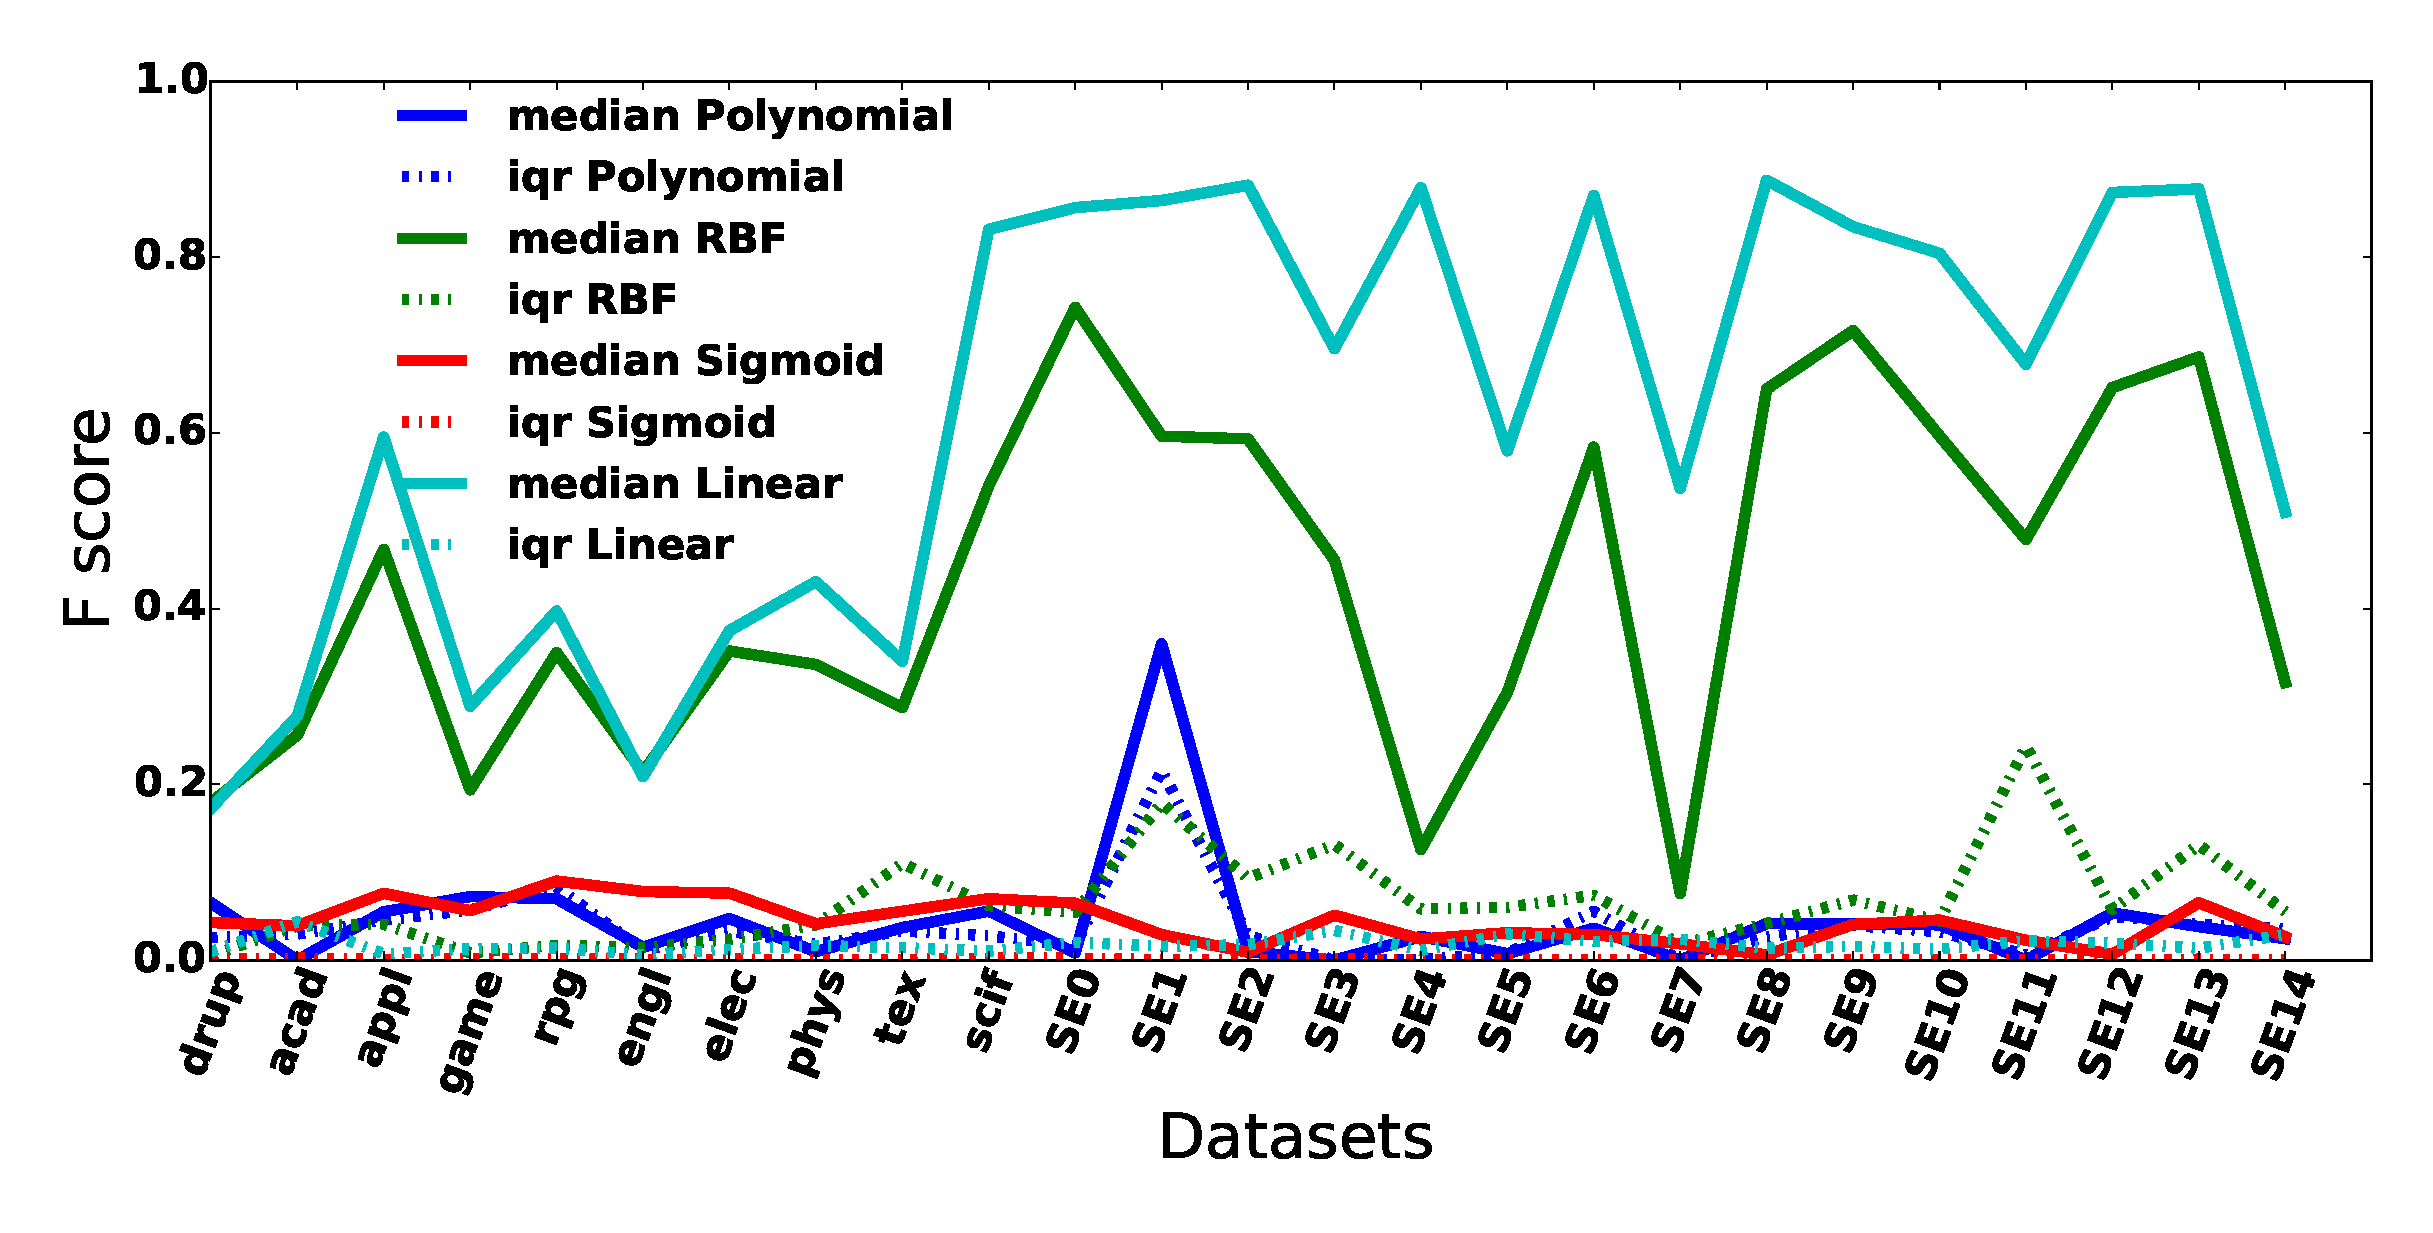
\includegraphics[width=0.48\linewidth]{./fig/algms2.eps}
        \label{fig:algms2}
    }
    \caption{Comparisons}
    \label{fig:all}
\end{figure*}

\subsection{Tokenization}

Tokenization is the very first step in natural language processing. It removes the spirit of symbols by identifing the most basic units which need not to be decomposed in the subsequent processing \cite{webster1992tokenization}. 

\textbf{Bag of words} is the tokenizer which simply splits each document into a group of single words. This is the most fundamental and costless tokenization in nature language processing.

\textbf{Shingling} introduces phrases as unit token. A word-based $w$-grams shingling captures contiguous sequences of words as unit tokens and each unit token has $w$ words \cite{chang2009using}.

\textbf{Stemming and stop words removal} combines words that have same meaning and removes meaningless words. It is considered as an effective way to improve the text classification performance \cite{yang1997comparative}. However contradictory evidences show that in the task of predicting tags, Stemming and stop words removal are not preferred \cite{moharanatag,stanley2013predicting}. An example of stemming and stop words removal is

\begin{equation*}
    \begin{aligned}
    &\textbf{Input: }"i\,want\,to\,eat\,apples\,since\,i\,like\,eating\,apples"\\
    &\textbf{Output: }"want\, eat\, appl\, sinc\, like\, eat\, appl".
    \end{aligned}
\end{equation*}


% \begin{figure}[ht]
%   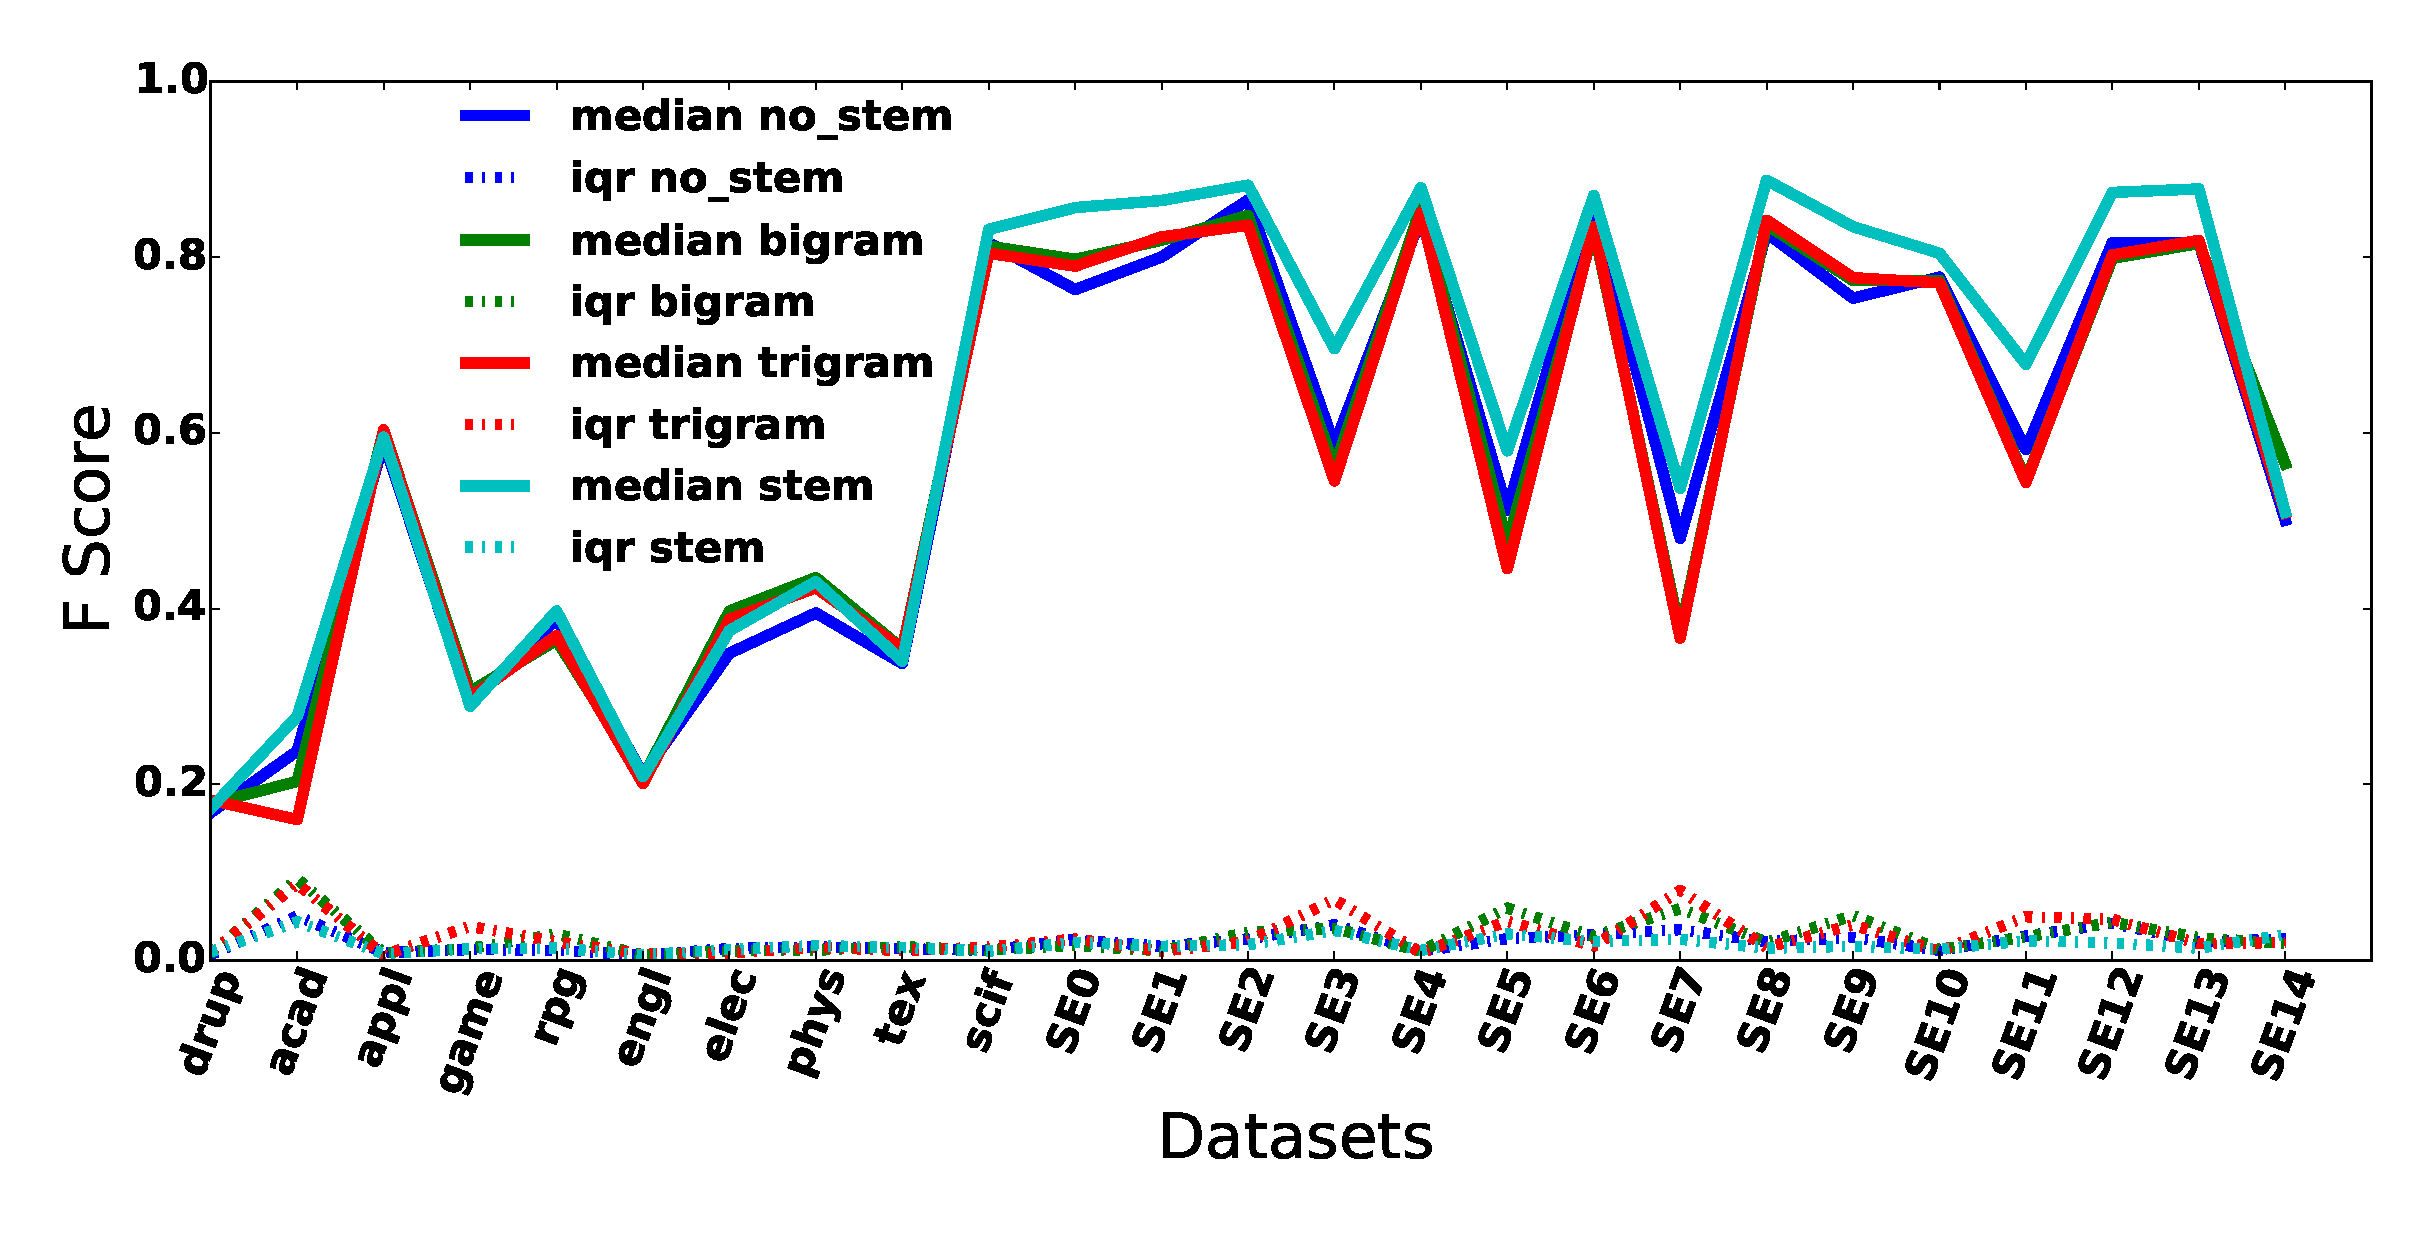
\includegraphics[width=\linewidth]{./fig/pre.eps}
%   \caption{Tokenization}
%   \label{fig:pre}
% \end{figure}


\textbf{Surprising fact:} Shingling does not help at all in our data, for our goal, while stemming only improves the performance a little bit. 

As shown in Figure \ref{fig:pre}, the average improvement of stemming and stop words removal in median value is 0.01 on tag-level data sets and 0.06 on site-level data sets. The average iqr of stemming and stop words removal improvement is 0.03 on tag-level data sets and 0.04 on site-level data sets. Given the fact that stemming and stop words removal does not introduce much cost in processing, it is recommended for our site-level prediction task.

\subsection{Featurization}

Featurization is the process which transforms the tokens of each document into a vector of weights of each unique token, which can be used to train the classifier. The top two most commonly used methods are compared in this experiment \cite{manning1999foundations}. 

\textbf{Term frequency }also known as word count, is the most commonly used and most fundamental feature weight in text categorization. \cite{manning1999foundations}. An example of this process is 

\begin{equation*}
\begin{aligned}
    &\textbf{Input: }[want\, eat\, appl\, sinc\, like\, eat\, appl]\\
    &\textbf{Output: }\{eat: 2,\, appl: 2,\, want: 1,\, sinc: 1,\,like: 1\}.
\end{aligned}
\end{equation*}

\textbf{Tf-idf weight }calculates not only the word count, but also the number of documents each token appears in. The basic idea of tf-idf weight is that the more frequent a token appears and the less documents it appears in, the more important it is. Tf-idf weight is also a popular feature for text categorization\cite{caropreso2001learner} and it is suggested in \cite{moharanatag} that better performance can be achieved with it. The tf-idf weight implemented in this experiment is:

\[\mathit{tfidf}(t, d) = |t  \in d| \cdot  log\left(\frac{|D|}{|d\in D: t\in d|}\right)\]
where $D,T$ are all documents and tokens and $t\in T,d\in D$.

% \begin{figure}[ht]
%   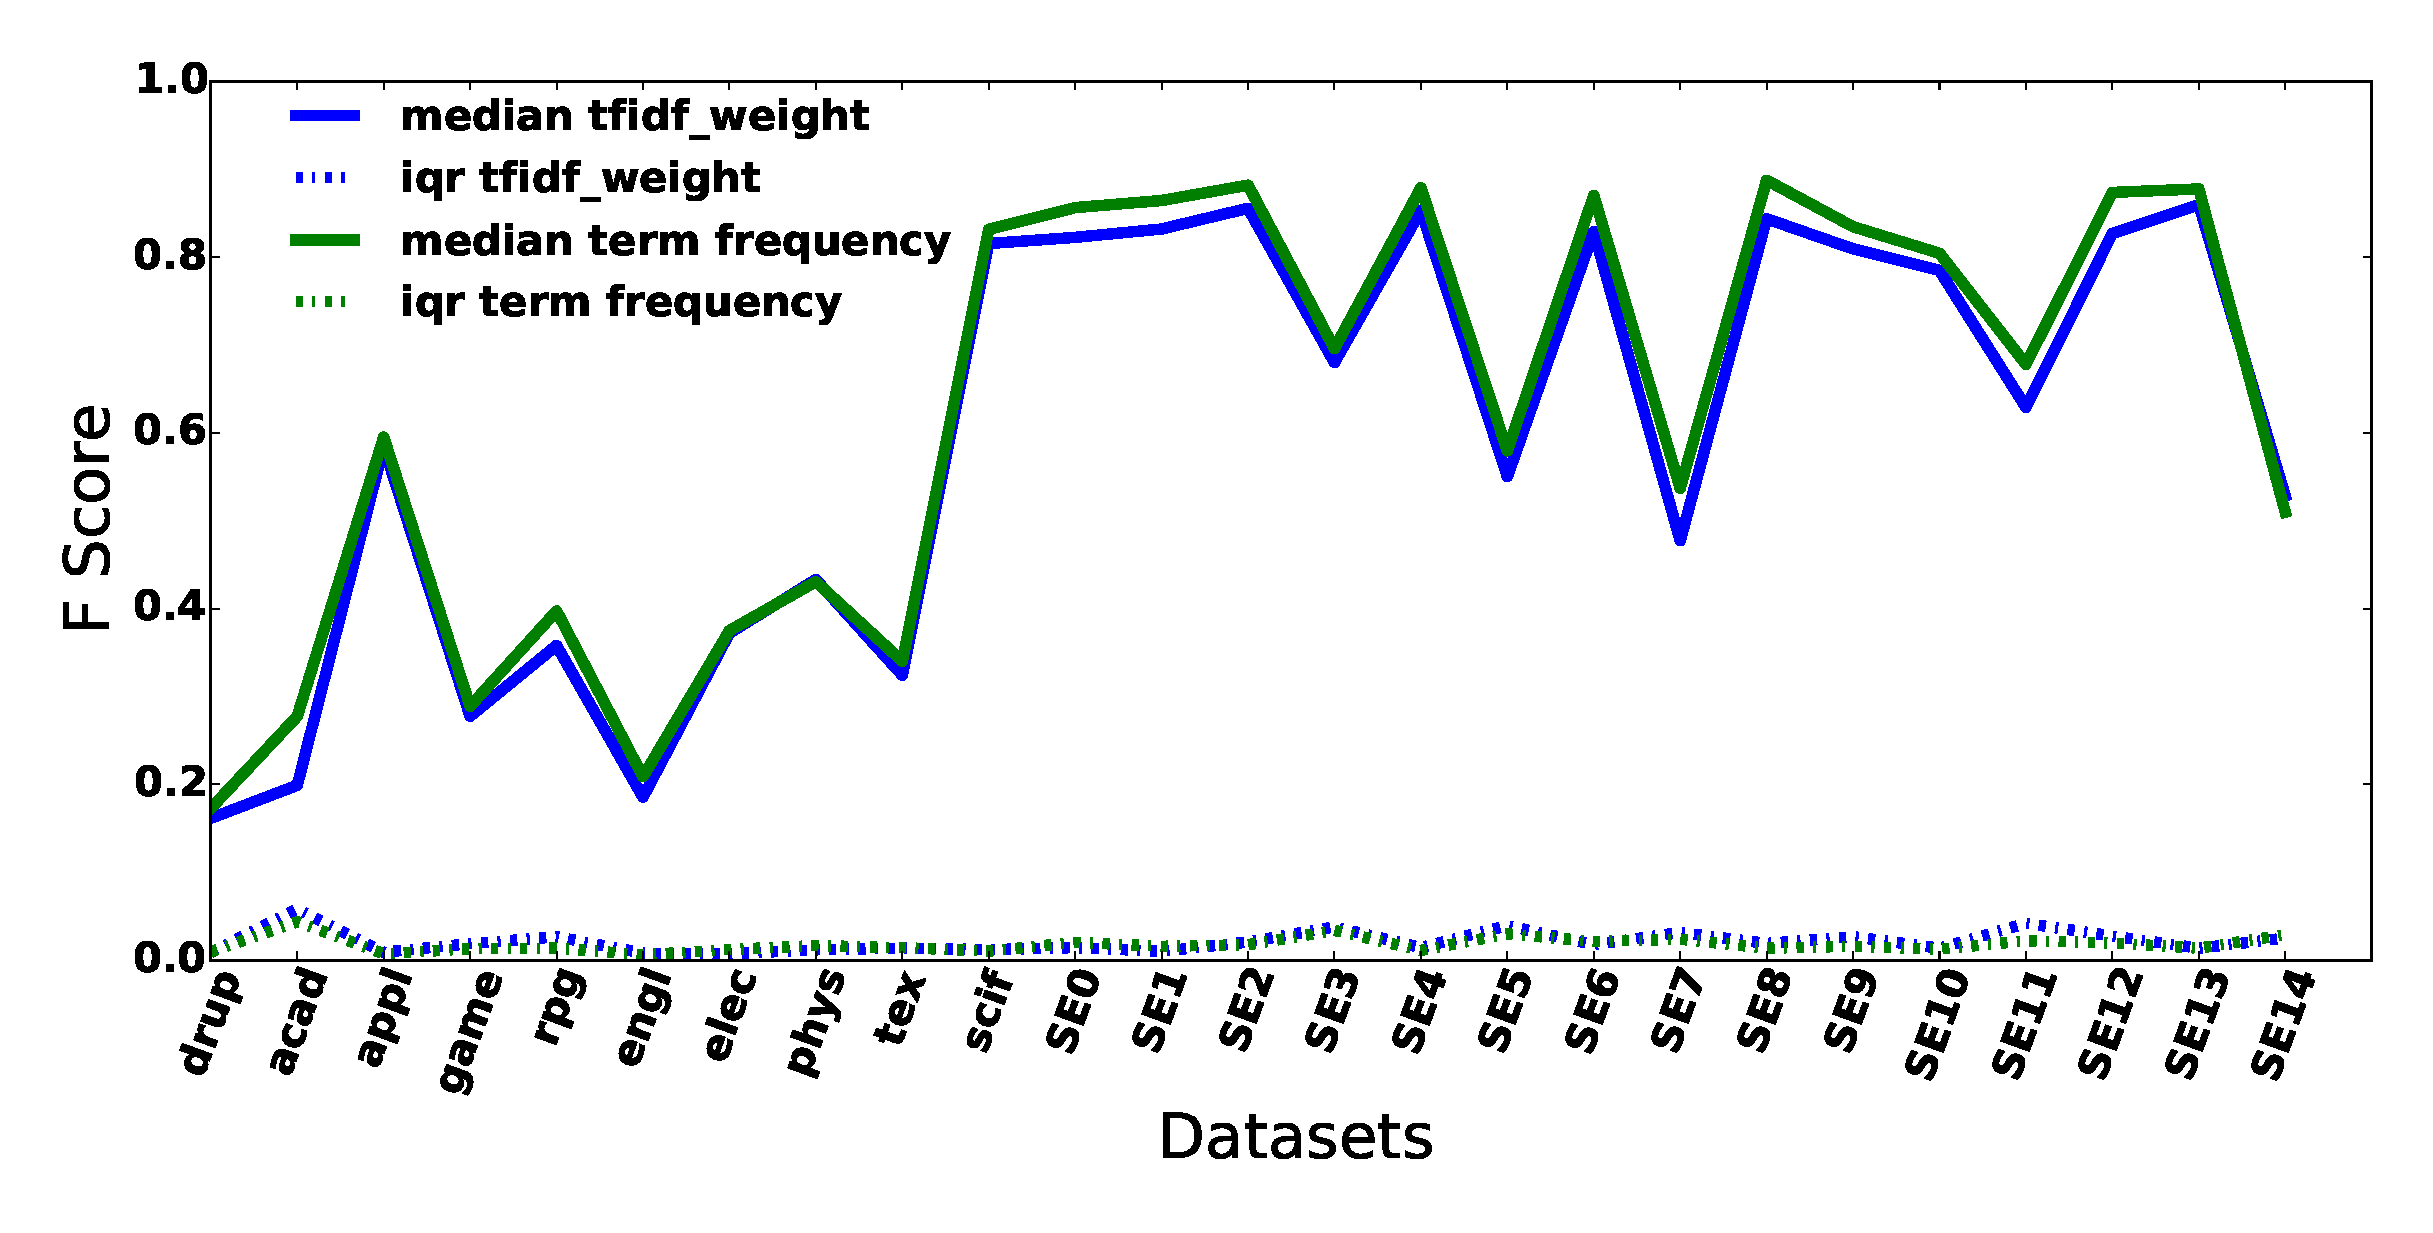
\includegraphics[width=\linewidth]{./fig/fea.eps}
%   \caption{Term frequency vs tf-idf weight}
%   \label{fig:fea}
% \end{figure}

\textbf{Surprising fact:} tf-idf weight performs no better than term frequency in our data, for our goal. 

As shown in Figure \ref{fig:fea}, term frequency performs even slightly better than tf-idf weight. Therefore term frequency is recommended for featurization due to its simplicity comparing with tf-idf weight.

\subsection{Dimensionality Reduction}

\begin{figure}[ht]
  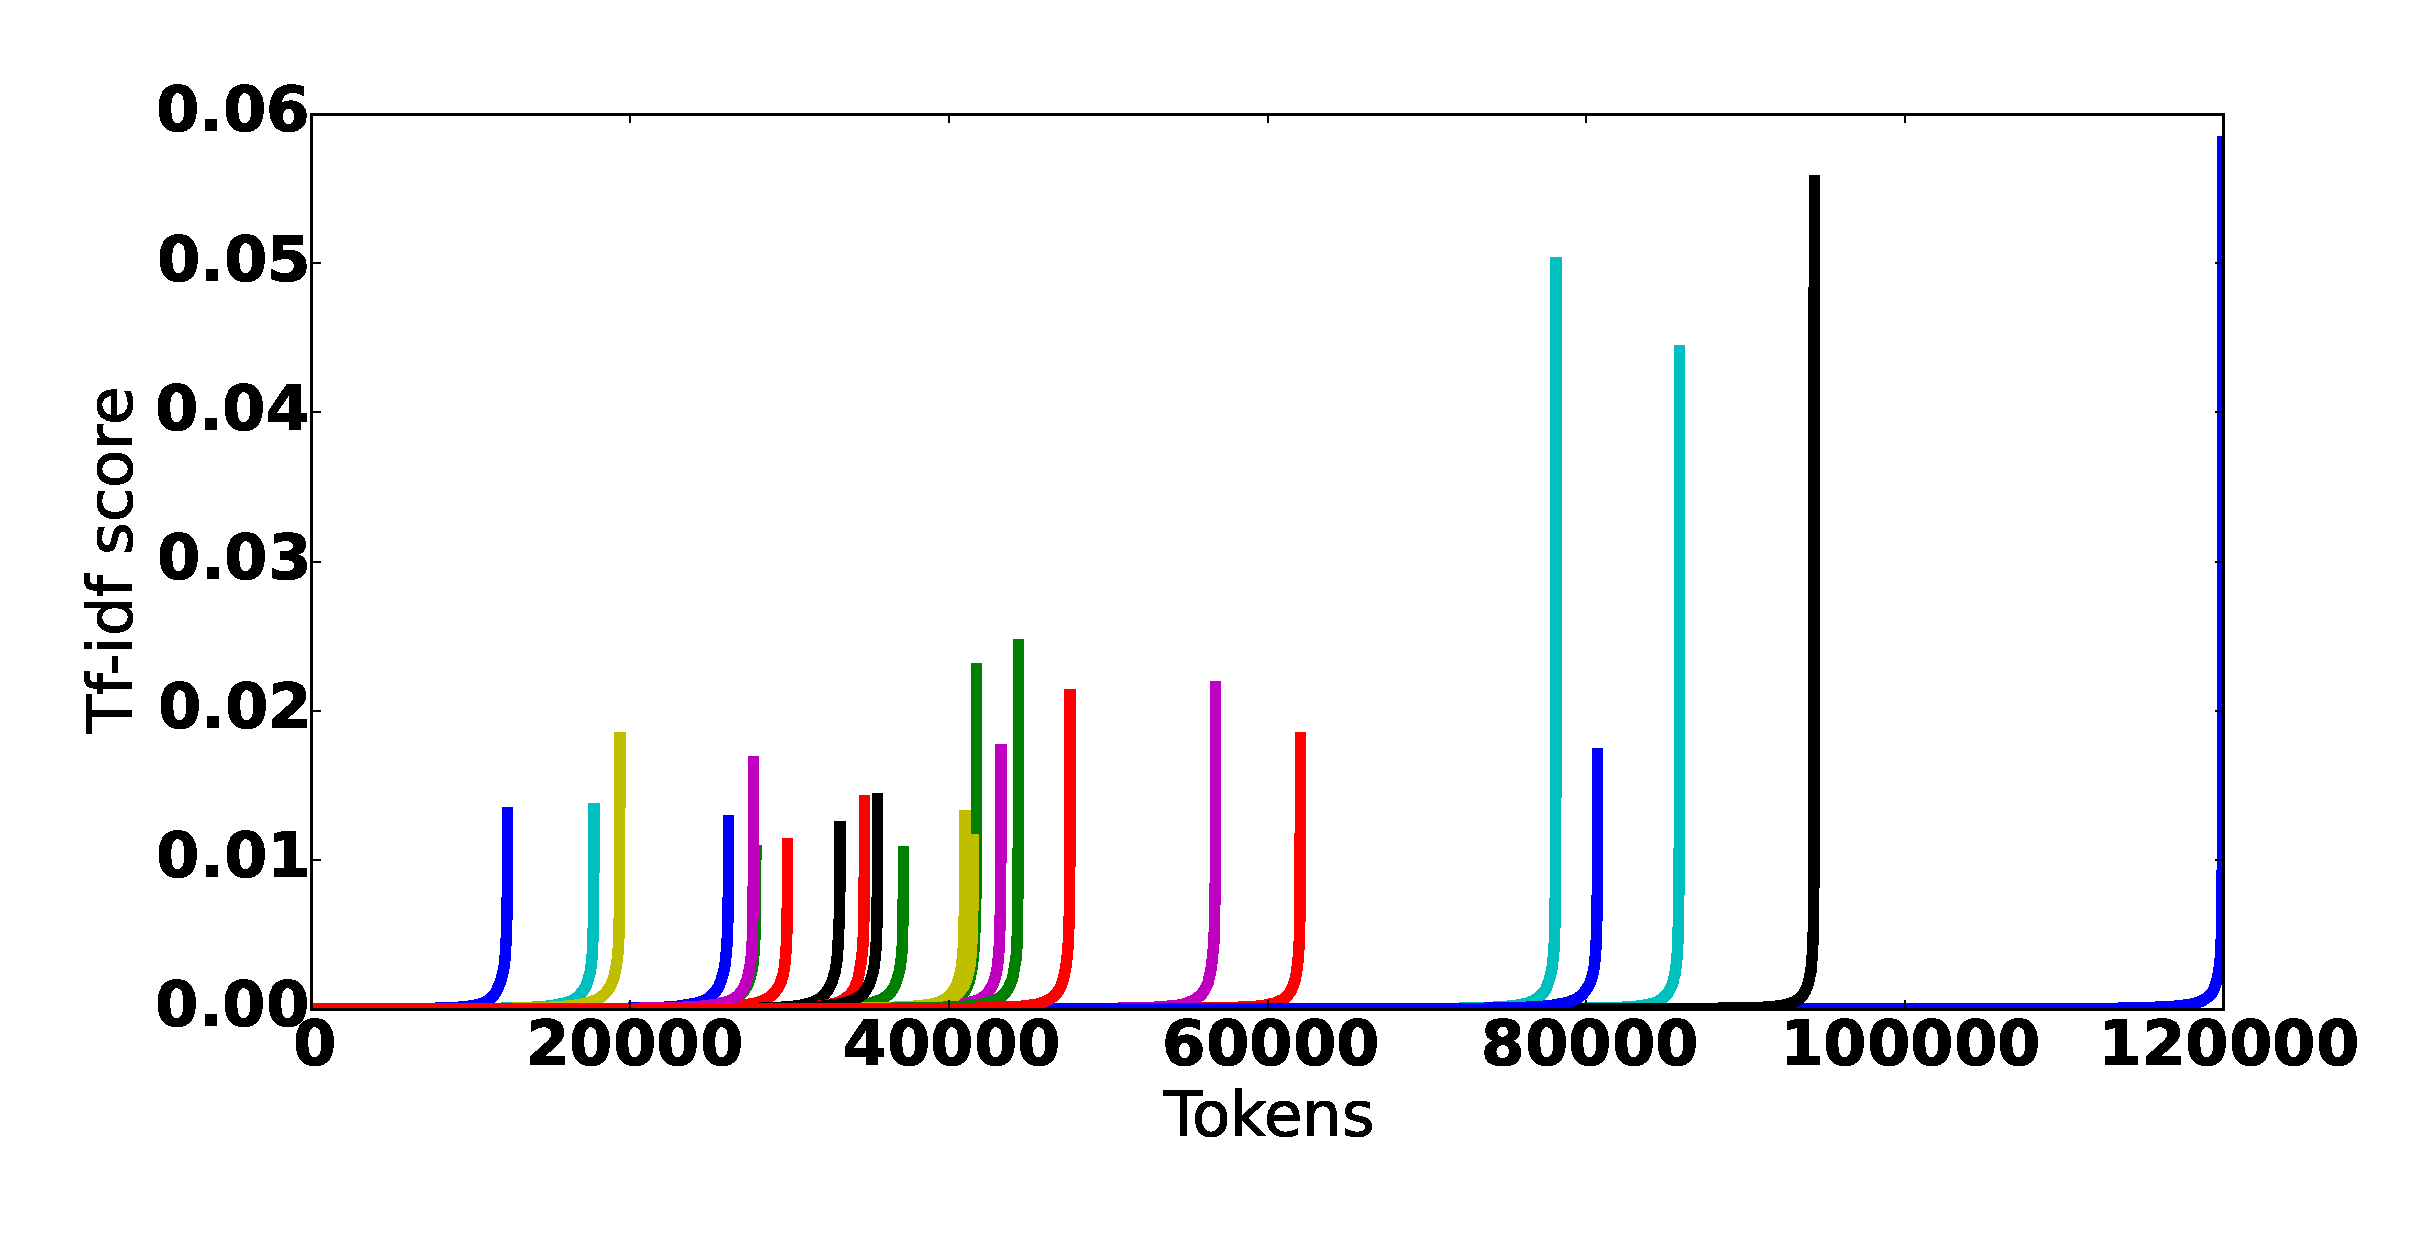
\includegraphics[width=\linewidth]{./fig/tokens.eps}
  \caption{Information of tokens}
  \label{fig:tokens}
\end{figure}

Dealing with the tables of data containing all the words in English, would mean processing a very large number of columns. A useful method for removing noise and reducing the computational costs in learning is dimensionality reduction. An example is shown in Figure \ref{fig:tokens} where tens of thousands of unique tokens exist in each data set and only a small number of those contain the most information. 

\textbf{Hashing trick} is a single-parse method that turns features into indices of in a matrix by applying a hash function to the features. The number of columns of the output matrix can be pre-defined and thus dimensionality reduction can be done by applying hashing trick \cite{weinberger2009feature}. An example of hashing trick is

\begin{equation*}
\begin{aligned}
    &\textbf{Input (N=3): }\{eat: 2,\, appl: 2,\, want: 1,\, sinc: 1,\,like: 1\}\\
    &\textbf{Output: }[3 \, 3 \, 1].
\end{aligned}
\end{equation*}

\textbf{Feature selection by tf-idf score} is also discussed in literature as an excellent method for text categorization \cite{menzies2006improving}. The idea is to sort tokens by their tf-idf score and pick the $N$ largest tokens. The tf-idf score mentioned here is measured as

\begin{equation*}
\begin{aligned}
   &tfidf(Token \,i)=\\
   &\Sigma^{D}_{j=1} WordCount(Token\, i, Document \,j)\cdot\\
   &log\frac{D}{DocumentCount(Token\,i)}, 
\end{aligned}
\end{equation*}

where $D$ is the total number of documents.

% \begin{figure}[ht]
%   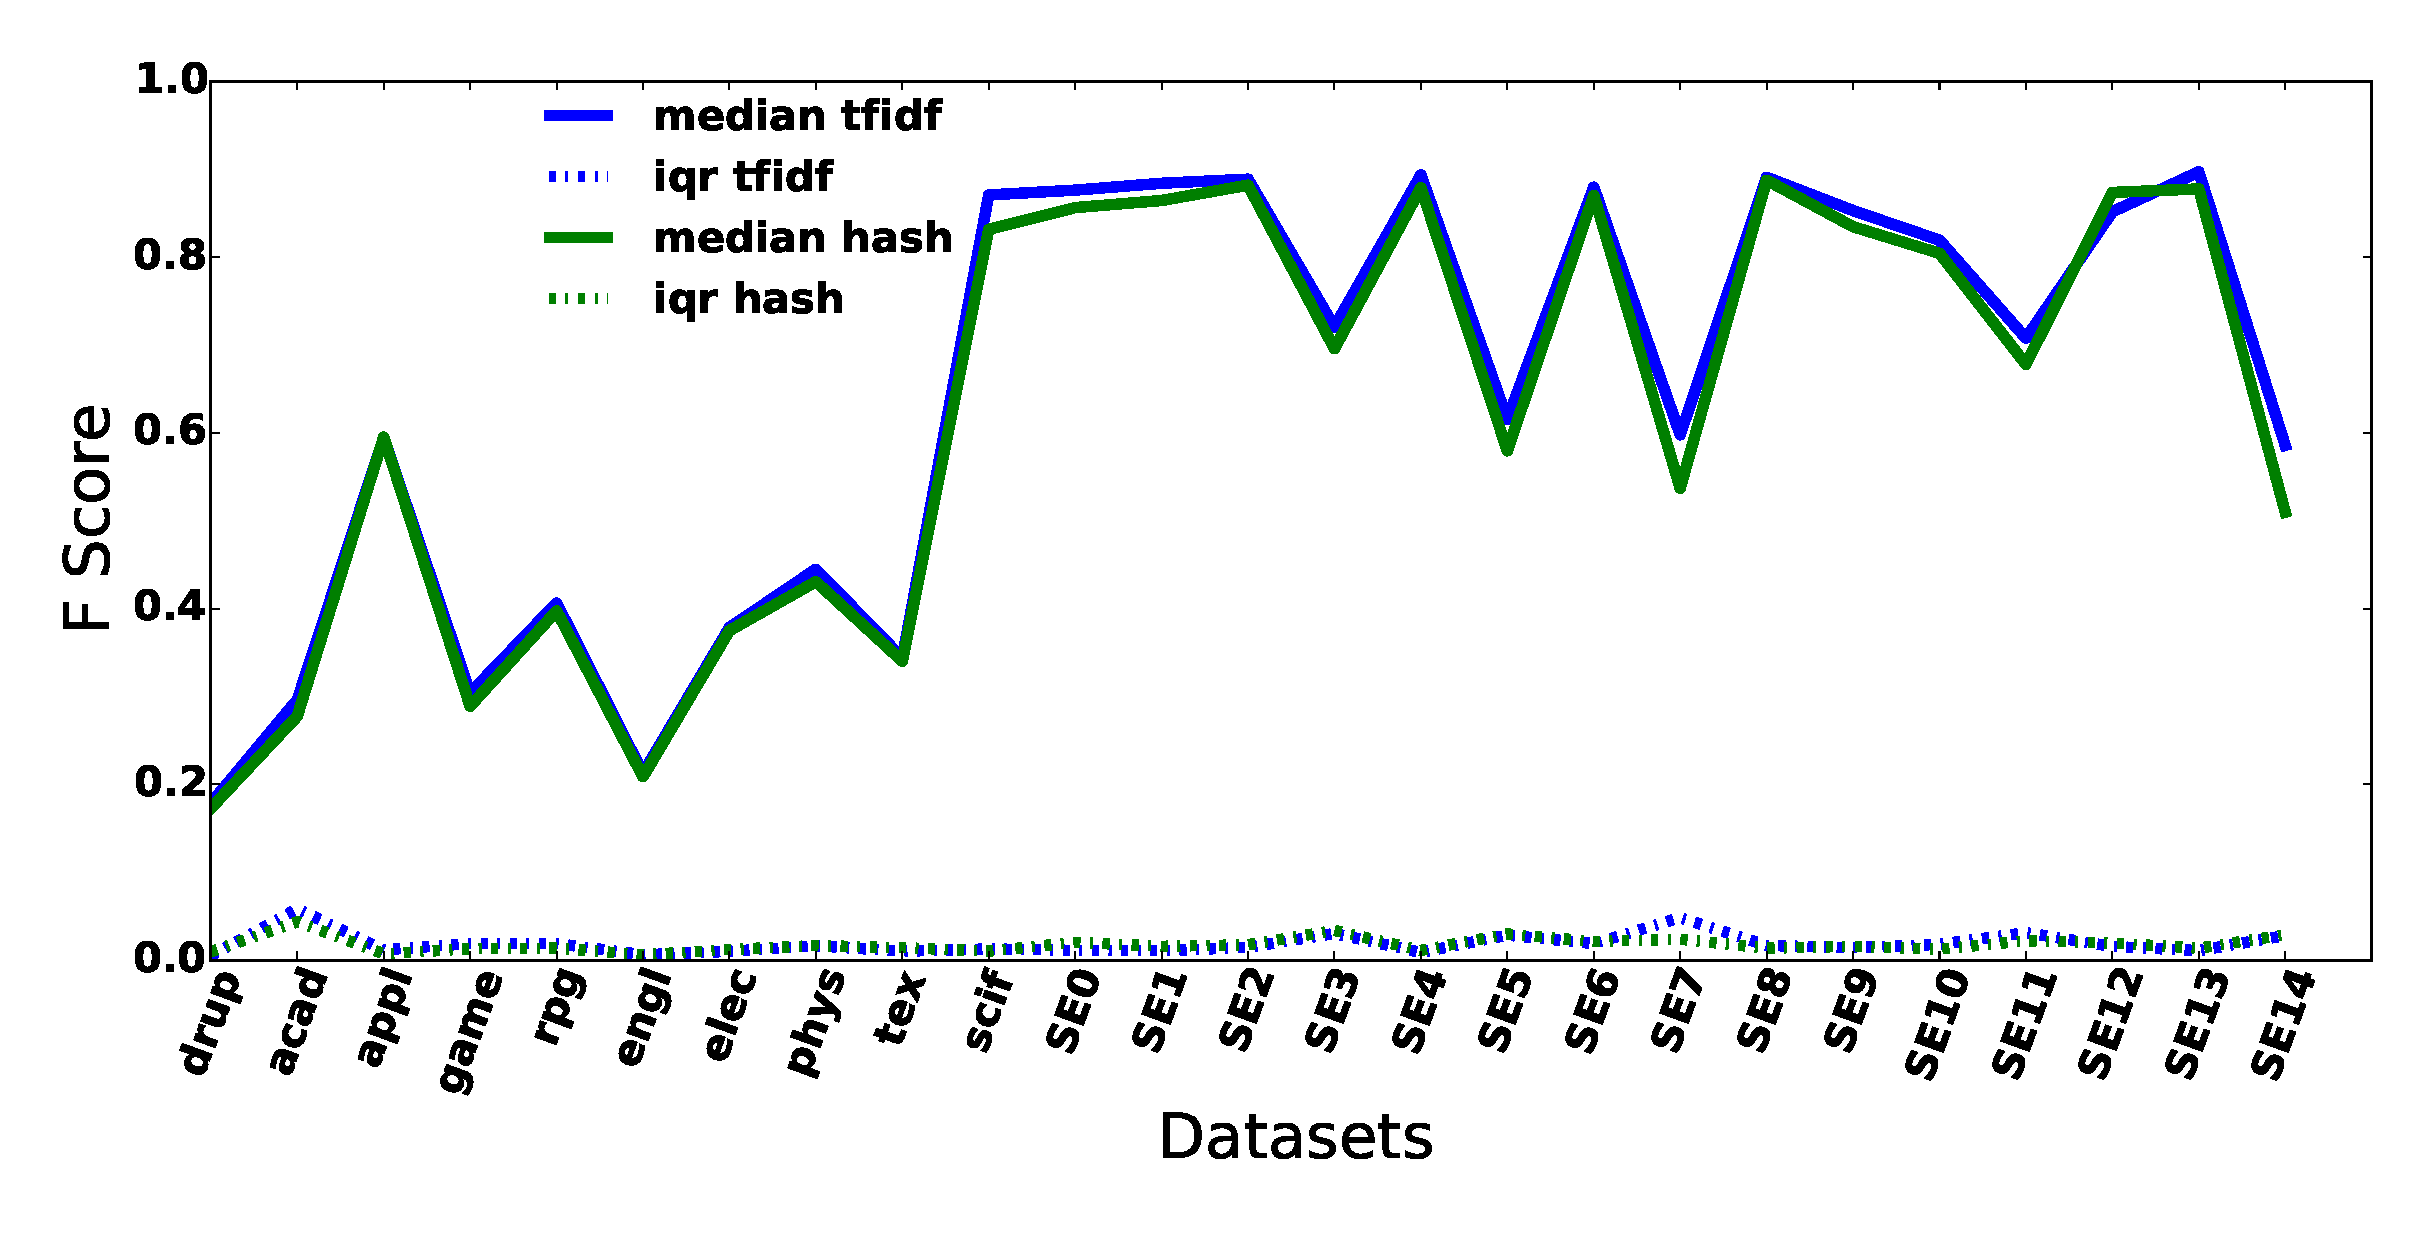
\includegraphics[width=\linewidth]{./fig/sel.eps}
%   \caption{Hashing vs tf-idf selection}
%   \label{fig:sel}
% \end{figure}

\textbf{Surprising fact:} the performances of tf-idf selection and hashing trick are almost the same. 

As shown in Figure \ref{fig:sel}, the differences of these two methods in median value is no bigger than the iqrs. Hashing trick is recommended due to its simplicity and high execution speed. 

% \begin{figure}[ht]
%   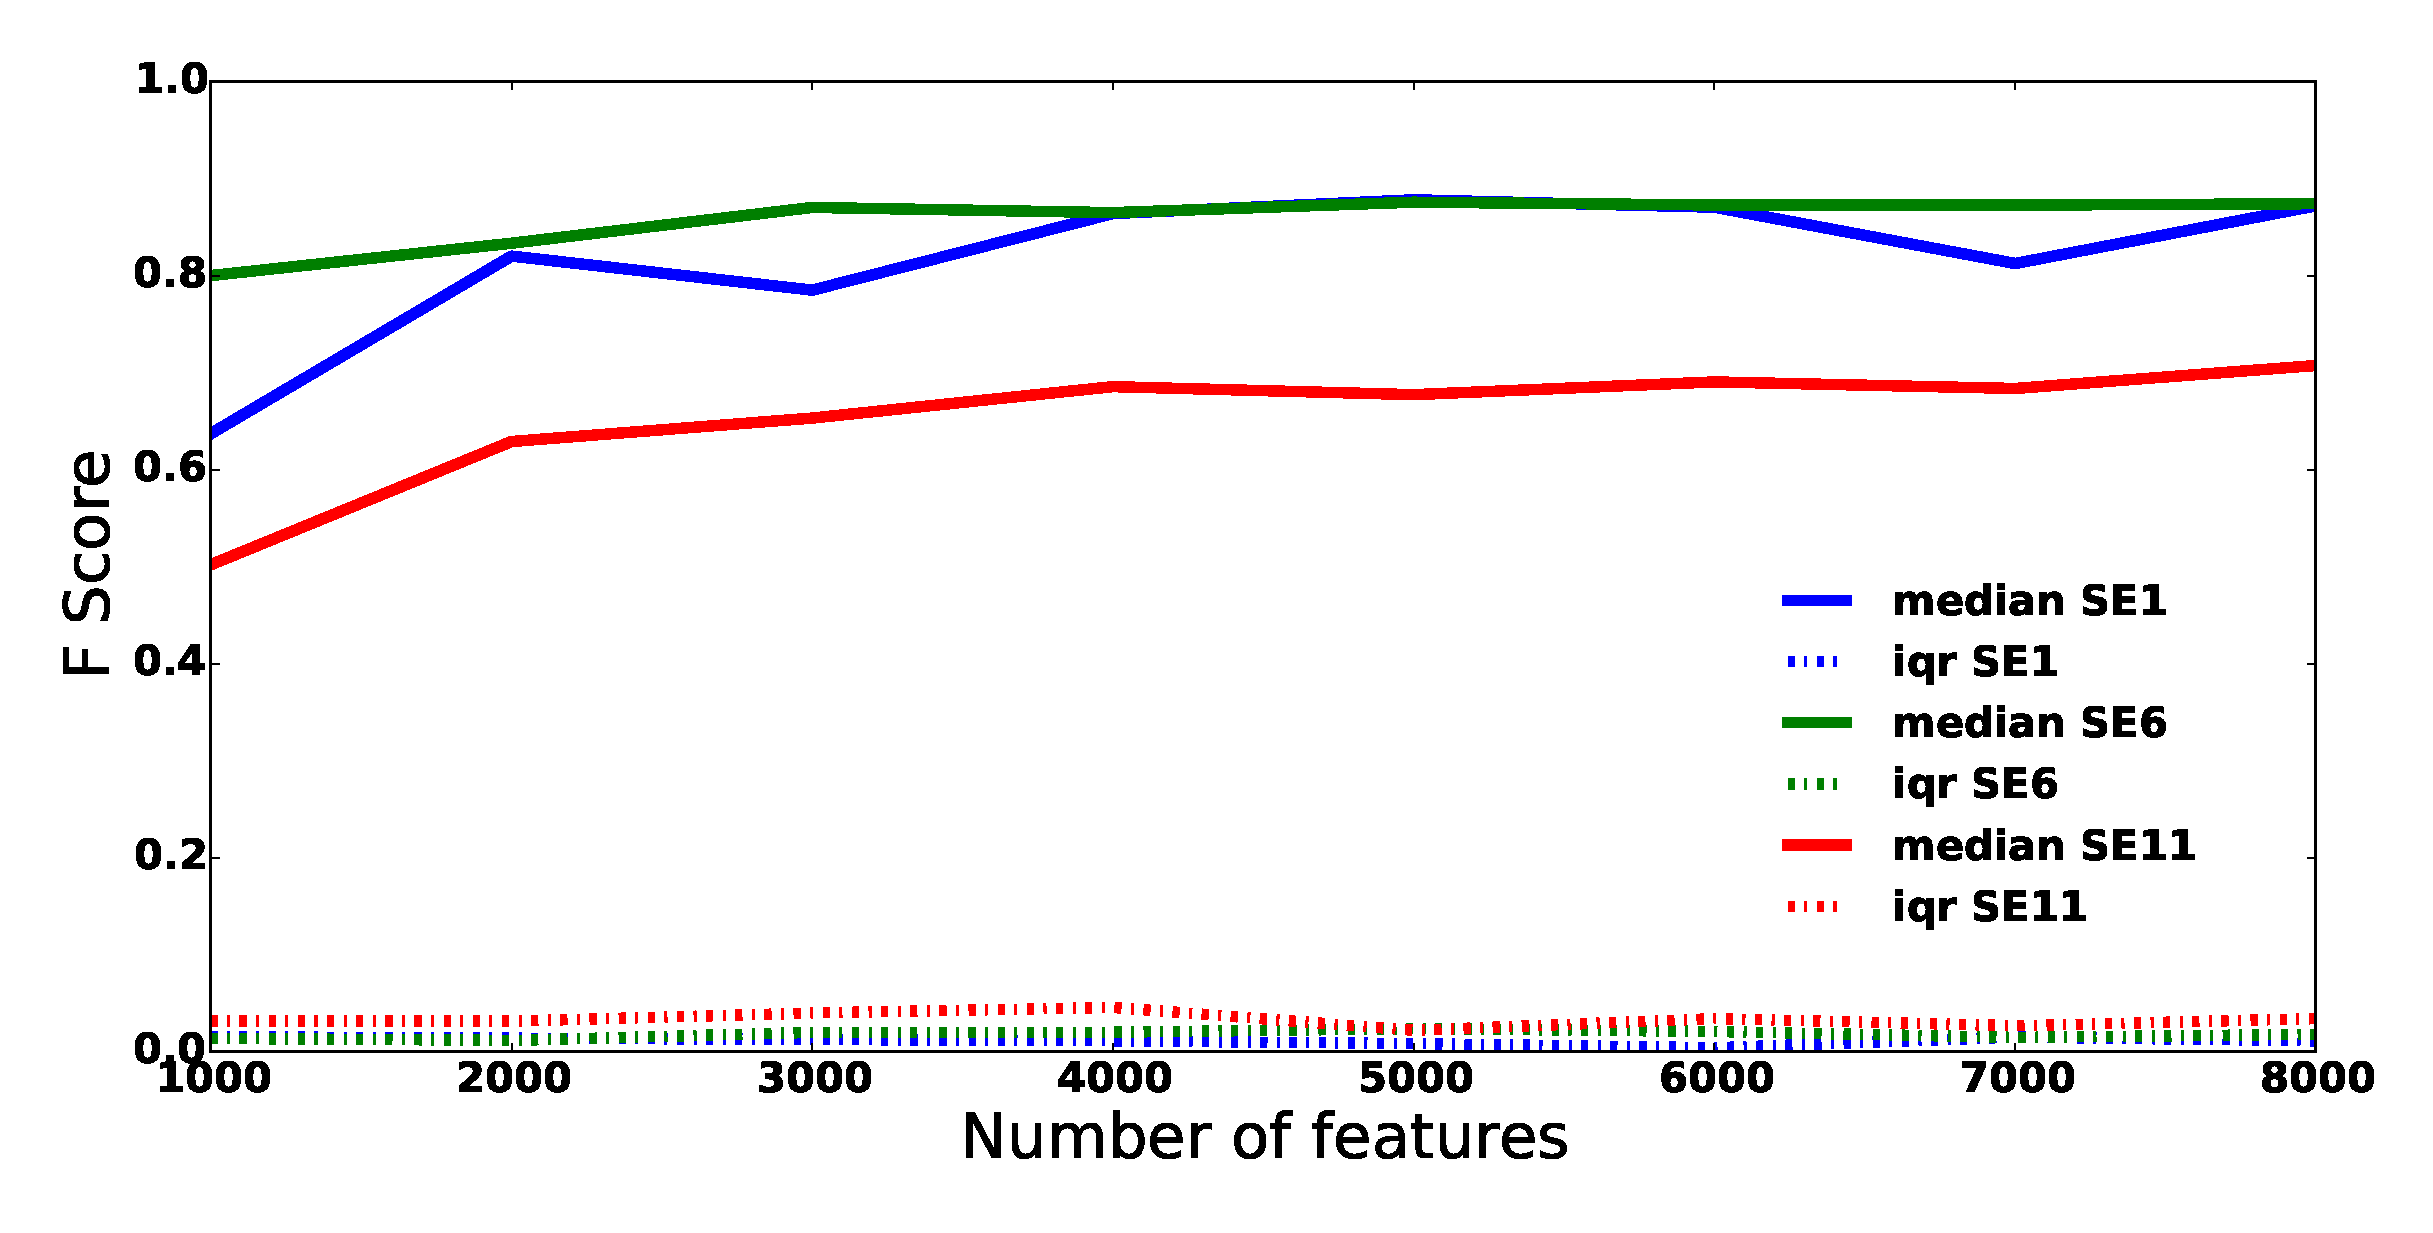
\includegraphics[width=\linewidth]{./fig/fea_num.eps}
%   \caption{Feature Numbers}
%   \label{fig:fea_num}
% \end{figure}

Additionally, learning curve shown in Figure \ref{fig:fea_num} suggests that the best number of features kept are $4000$. Results from only three data sets are presented in Figure \ref{fig:fea_num} due to the limited space. What we do not show is that in most of the 25 data sets, the elbow appears around 4000.

\subsection{Normalization}

Normalization is the process which adjust the values measured on different scales to a notionally common scale.

\textbf{L2 normalization on columns} grabs feature vector of each feature and divide it by its L2 norm. It is suggested by the definition of normalization. In general data mining tasks, the weight of different features are measured on different scales. Normalization on columns of the feature matrix eliminates these differences among features.

\textbf{L2 normalization on rows} grabs feature vector of each document and divide it by its L2 norm. It is the standard normalization method for text categorization \cite{frank2006naive}. The main purpose of implementing L2 normalization on rows is to rescale the vector of feature weights to unit length. An example of L2 normalization on rows is

\begin{equation*}
\begin{aligned}
    &\textbf{Input: }[3 \, 3 \, 1]\\
    &\textbf{Output: }[3 \, 3 \, 1]./\sqrt{(3^2+3^2+1^2)}=[0.69 \quad 0.69 \quad 0.23].
\end{aligned}
\end{equation*}

% \begin{figure}[ht]
%   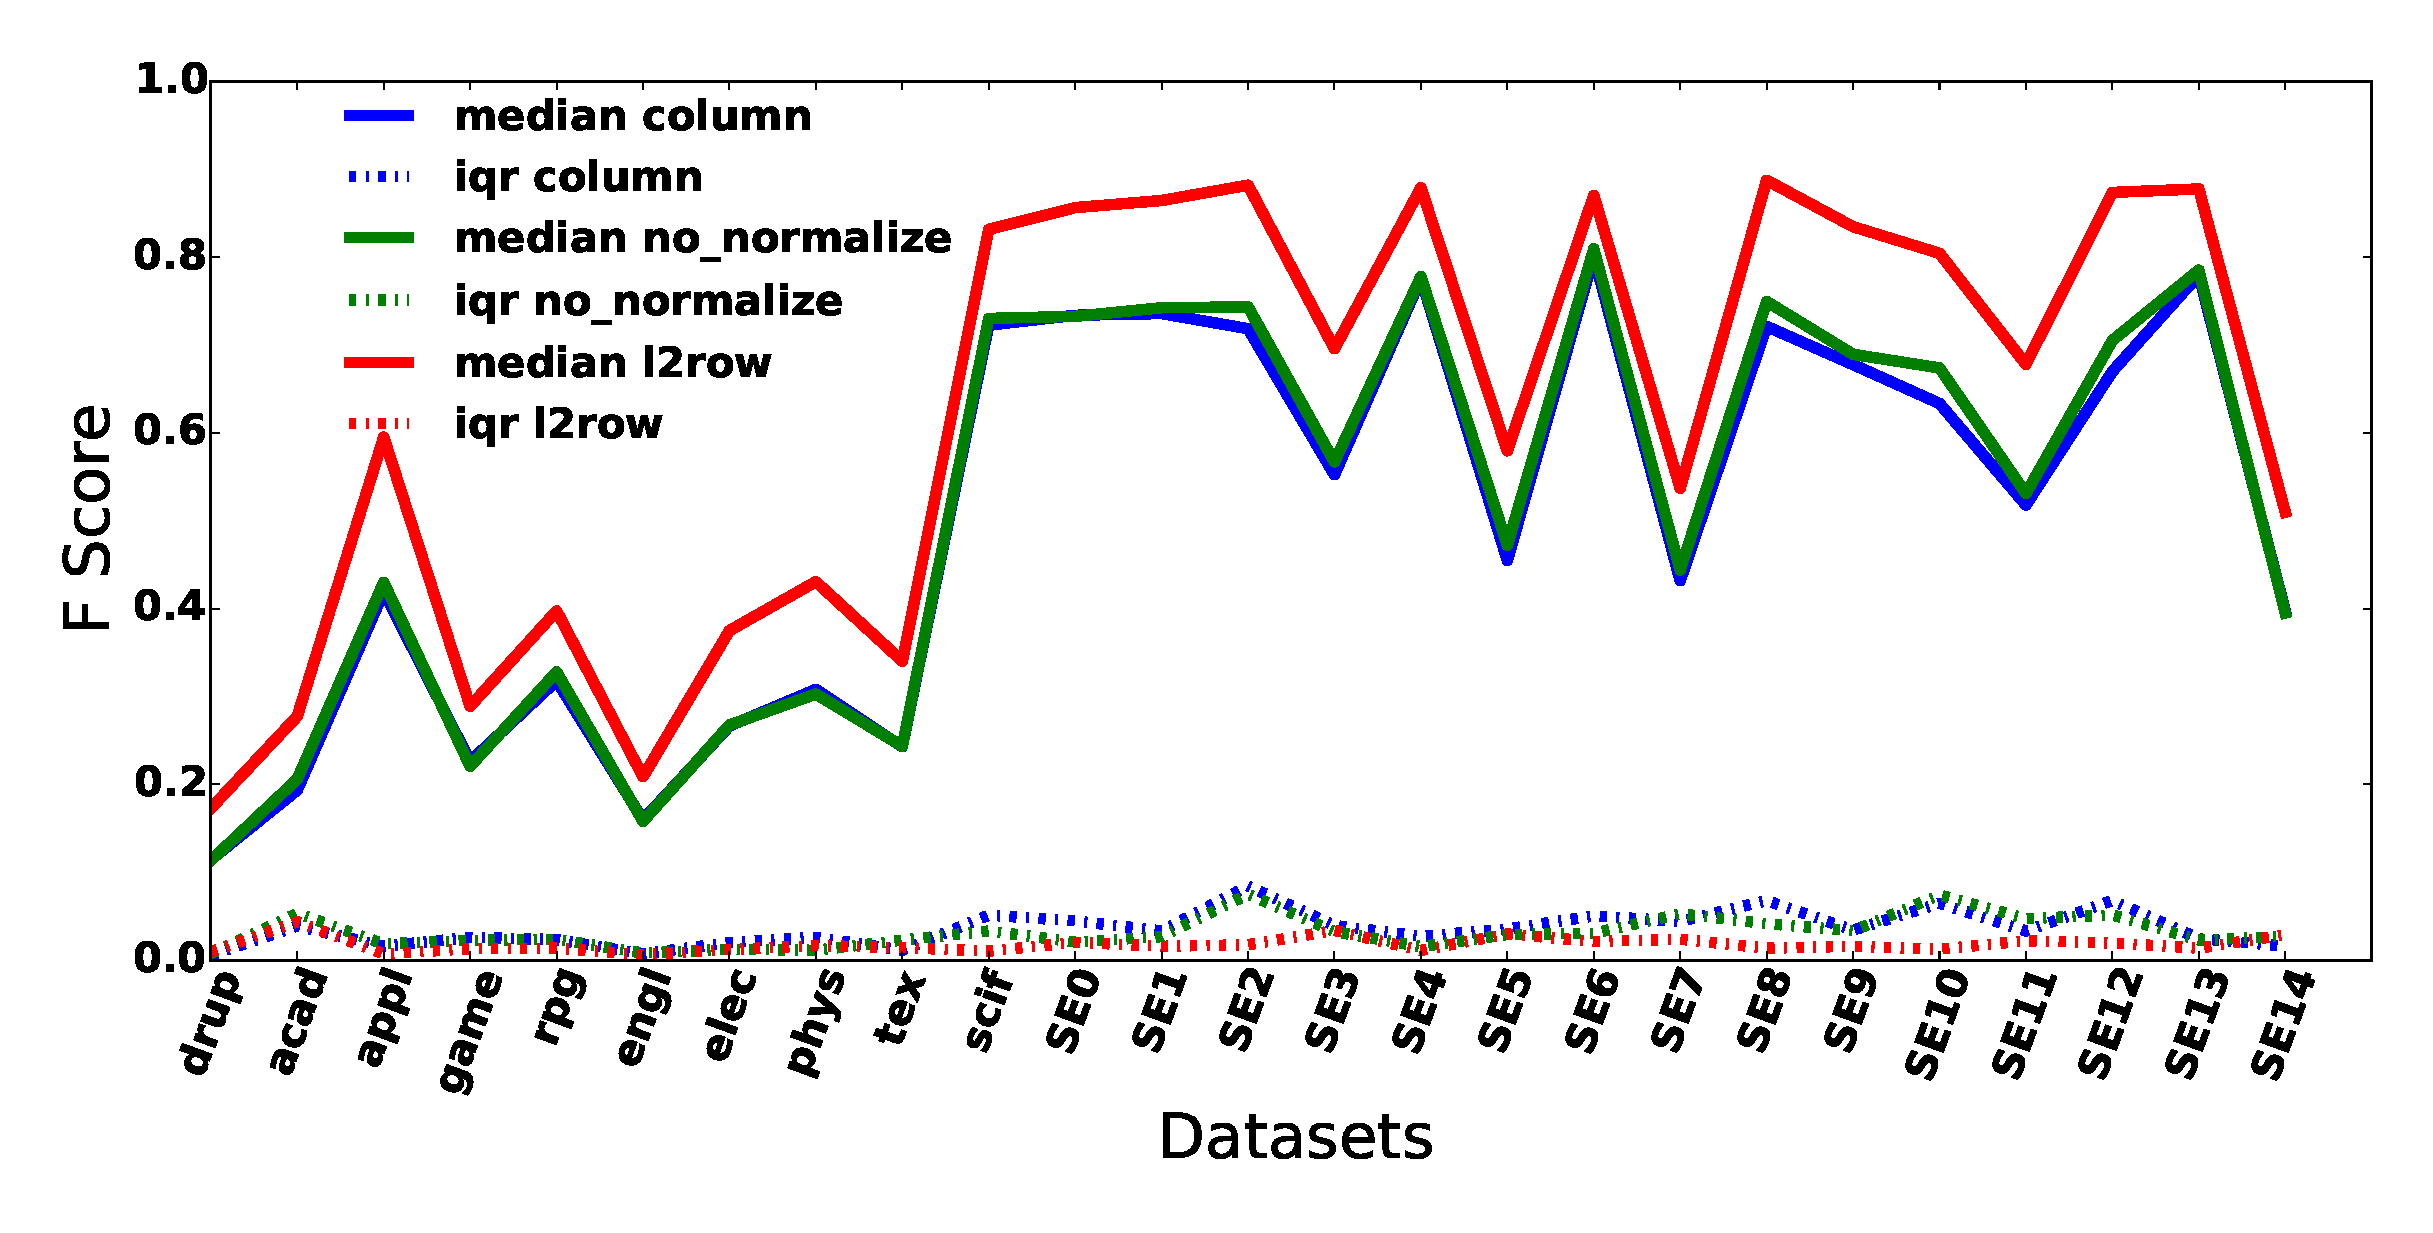
\includegraphics[width=\linewidth]{./fig/norm.eps}
%   \caption{Normalization methods}
%   \label{fig:norm}
% \end{figure}

\textbf{Not surprising fact:} L2 normalization on rows outperforms L2 normalization on columns and indeed improves the performance.

All the feature weights in our data are actually measured on same scales, therefore we expect no difference between L2 normalization on columns and no normalization. On the other hand, the length of documents in our data vary in a large scale and L2 normalization on rows helps to eliminate these differences.

As shown in Figure \ref{fig:norm}, there is no difference between L2 normalization on columns and no normalization. On the other hand, the average improvement of L2 normalization on rows in median value is 0.09 on tag-level data sets and 0.12 on site-level data sets. The average iqr of L2 normalization on rows improvement is 0.04 on tag-level data sets and 0.06 on site-level data sets. Therefore L2 normalization on rows is recommended for normalization.



\subsection{Data Balancing}
\label{sect:Data Balancing}

Data balancing may not be one of the standard process of text categorization, but is indispensable in our data. Given the fact that the population of "related" documents is usually only 2-5\% of the whole population, imbalance is a significant feature of the data. Data balancing is usually executed in two directions: over-sample the minority class while under-sample the majority class. In this experiment, we choose to under-sample the majority class by sampling without replacement while over-sample the minority class by SMOTE. The population of each class will be the same after data balancing.

\textbf{SMOTE} over-samples the minority class by introducing synthetic examples along the line segments joining any pair of real samples in neighborhood.  Proposed in 2002 \cite{chawla2002smote}, SMOTE is a very effective over-sampling method and has been widely applied during the past decades \cite{han2005borderline,bunkhumpornpat2009safe,luengo2011addressing}. 

% \begin{figure}[ht]
%   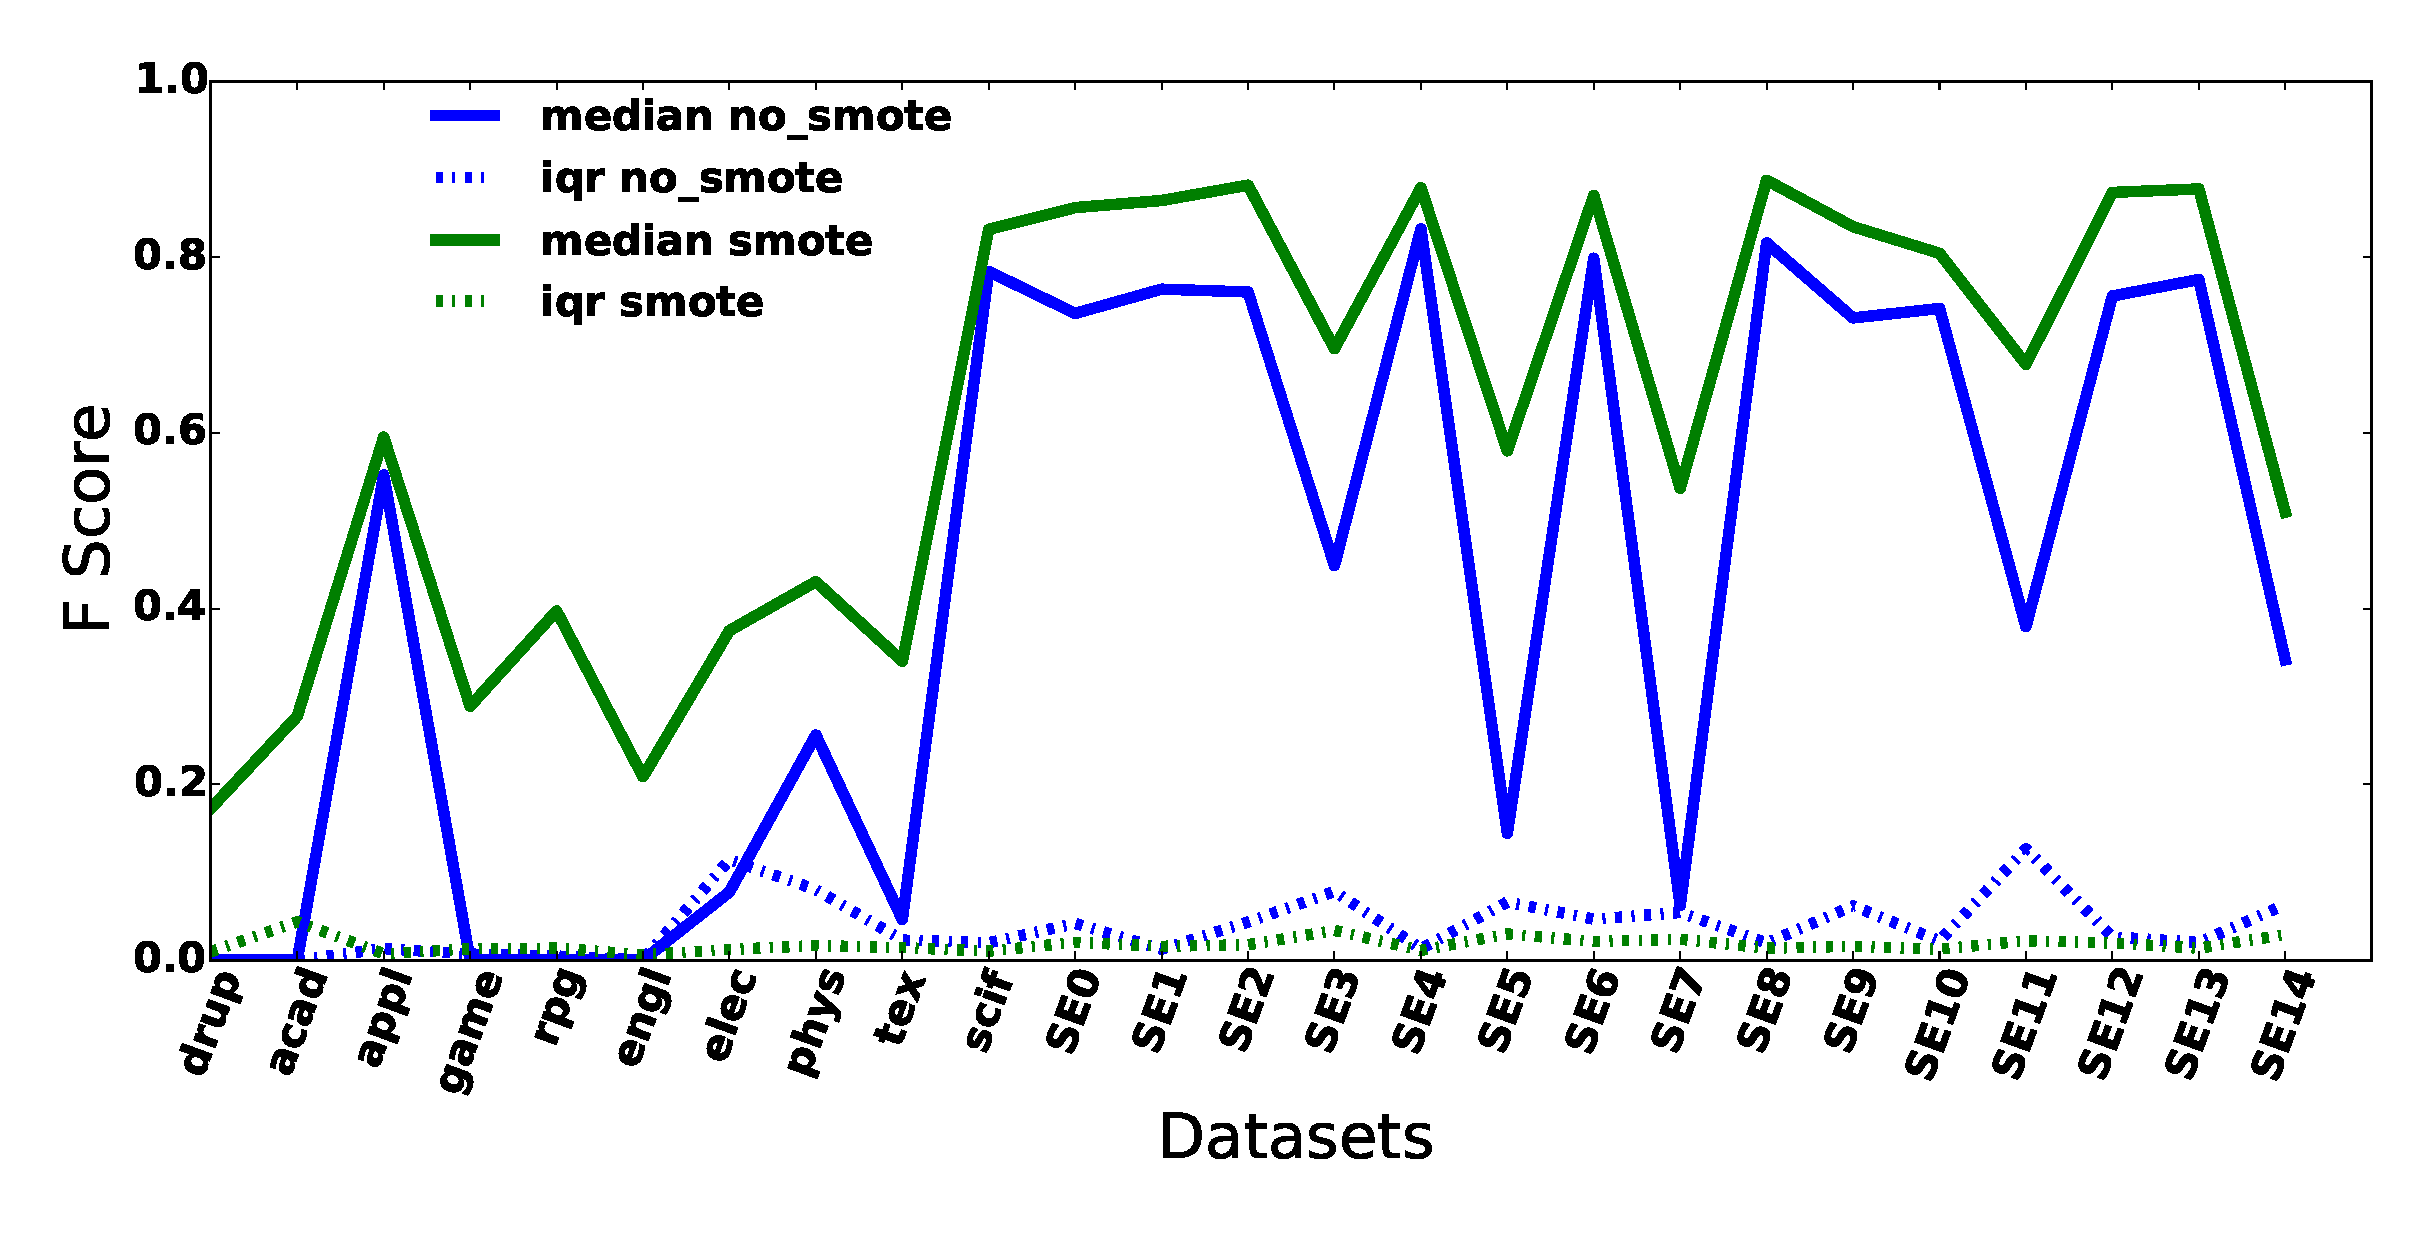
\includegraphics[width=\linewidth]{./fig/balance.eps}
%   \caption{SMOTE or not}
%   \label{fig:balance}
% \end{figure}

\textbf{Surprising fact:} SMOTE significantly improves the performance on both tag-level and site-level data sets.

As shown in Figure \ref{fig:balance}, the average improvement of SMOTE in median value is 0.22 on tag-level data sets and 0.17 on site-level data sets. The average iqr of SMOTE improvement is 0.04 on tag-level data sets and 0.07 on site-level data sets. Therefore SMOTE is absolutely necessary.

\subsection{Classification}

Classifier might be the most important decision of a data mining system. The three most fundamental and commonly used classifiers are compared in the following experiment.

\textbf{SVM} is one of the most famous supervised learning models for all data mining tasks. Linear SVM is especially considered effective in text categorization \cite{joachims2006training} and in predicting tags \cite{moharanatag}. 

\textbf{Naive Bayes} represents a family of simple probabilistic classifiers which has been studied extensively since 1950s. Multinomial Naive Bayes is especially designed for text categorization \cite{mccallum1998comparison} and always considered as a baseline method for text categorization. 

\textbf{Decision Tree} is also considered as a popular model for classification. CART is one implementation of decision tree model that has been proved to fit well in text categorization \cite{miotto2005supporting}.

% \begin{figure}[ht]
%   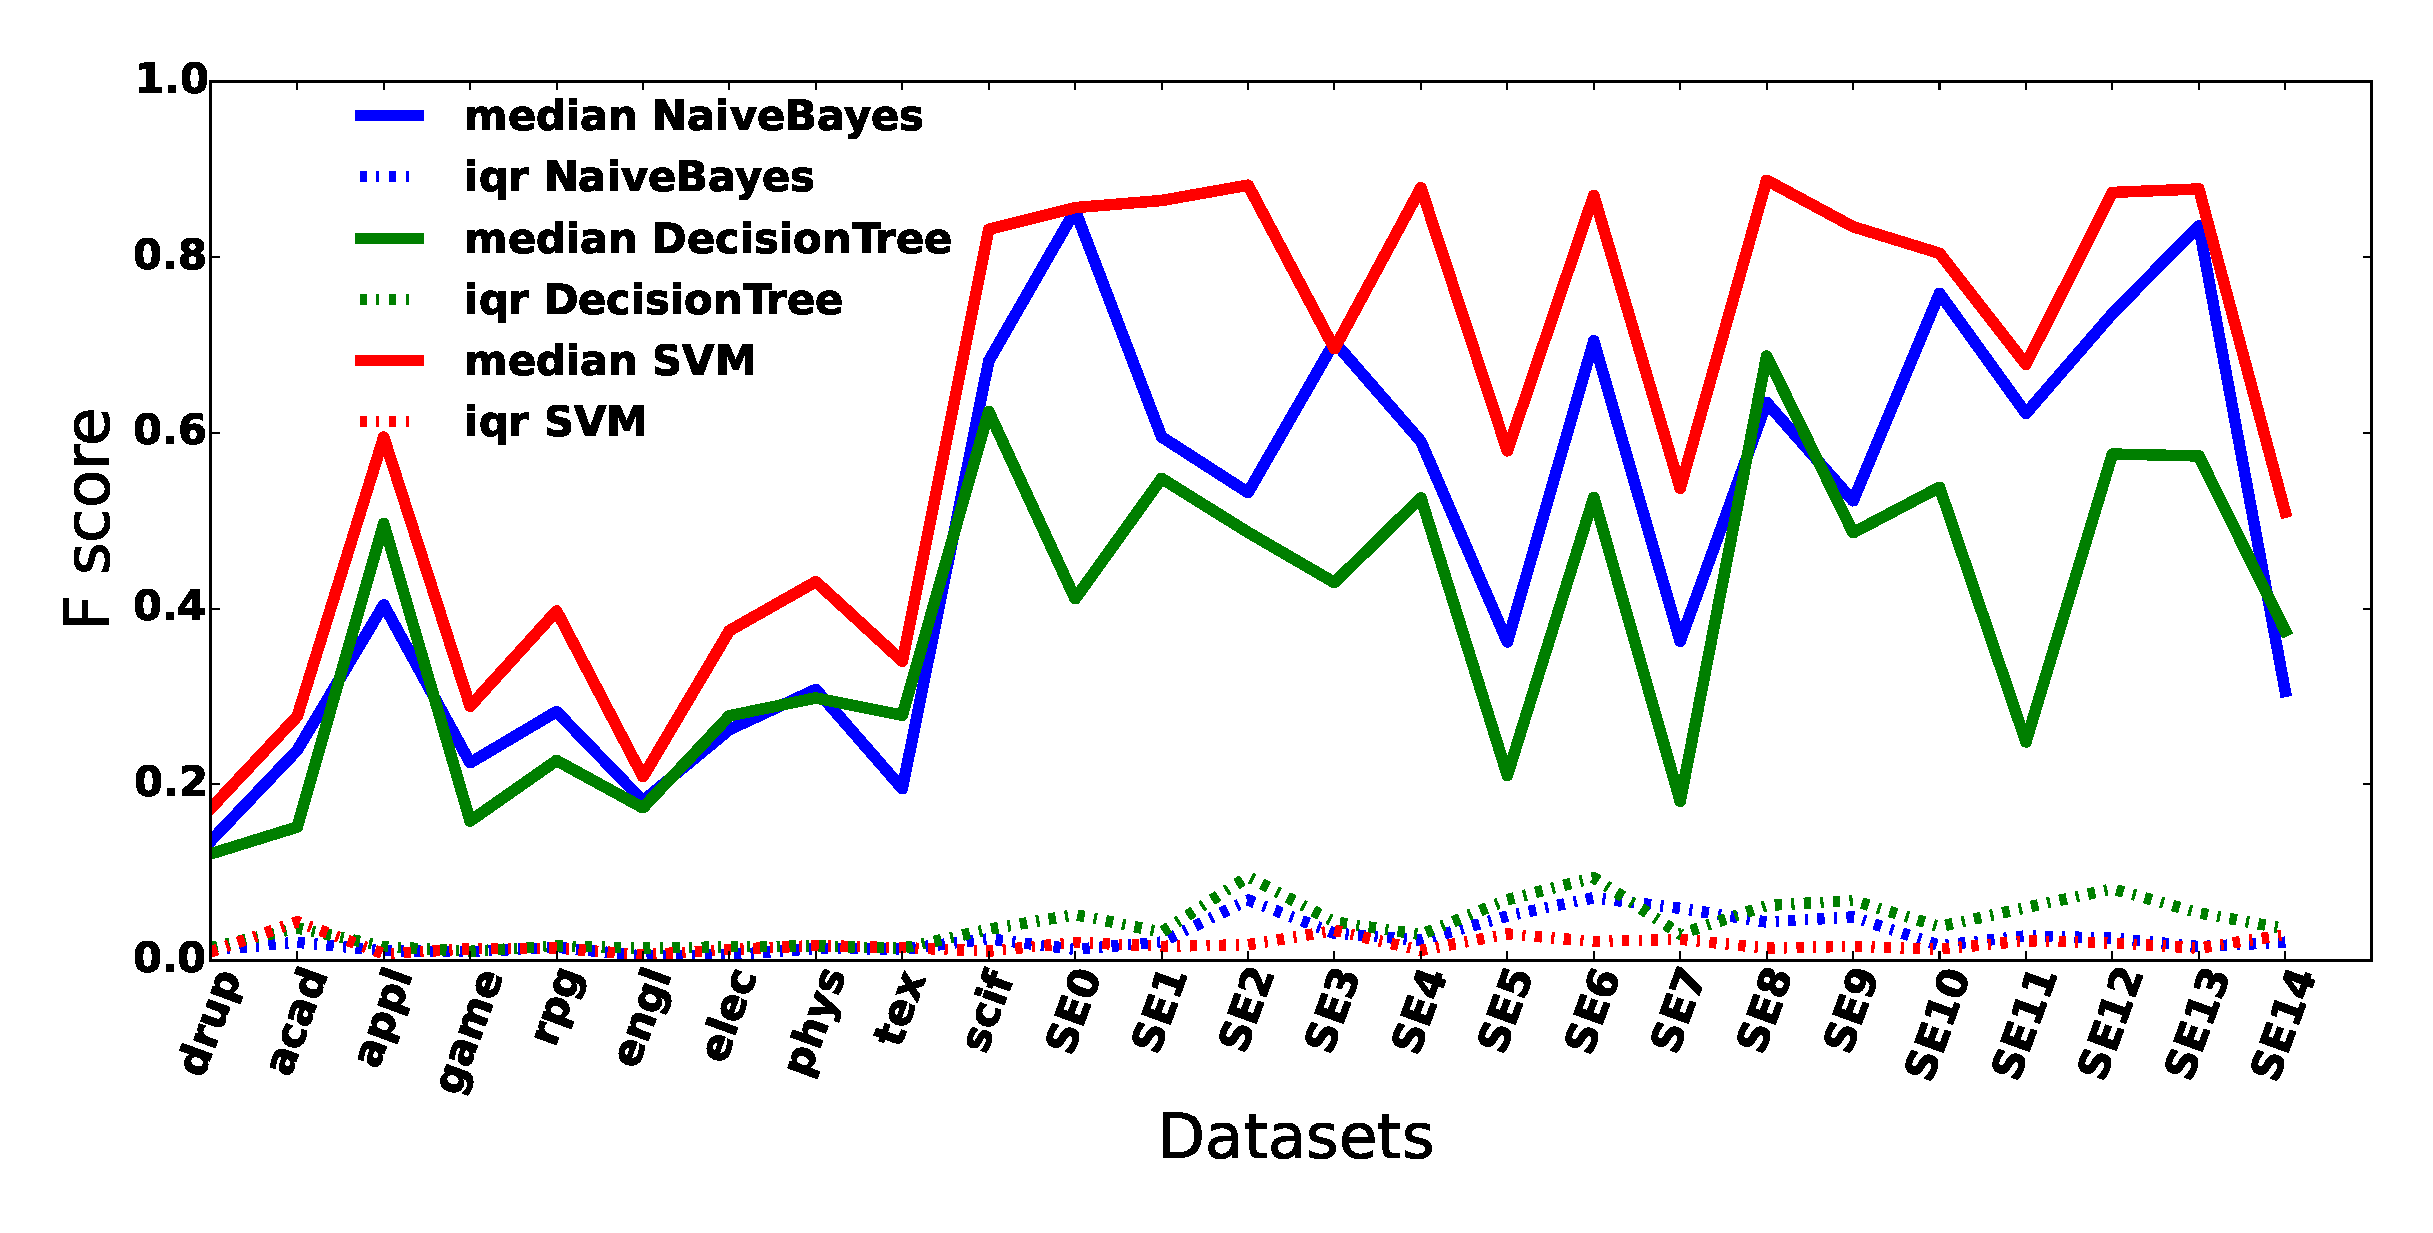
\includegraphics[width=\linewidth]{./fig/algms1.eps}
%   \caption{Classifiers}
%   \label{fig:algms1}
% \end{figure}

\textbf{Surprising fact:} linear SVM ourperforms the other classifiers a lot. Nonlinear kernels do not really help in our data, for our goal.

As shown in Figure \ref{fig:algms1}, linear SVM is always the best classifier in all the 25 data sets. Furthermore, we tested SVM with different kernels. With the result shown in Figure \ref{fig:algms2}, linear kernel is justified as the best kernel for SVM in this task.

% \begin{figure}[ht]
%   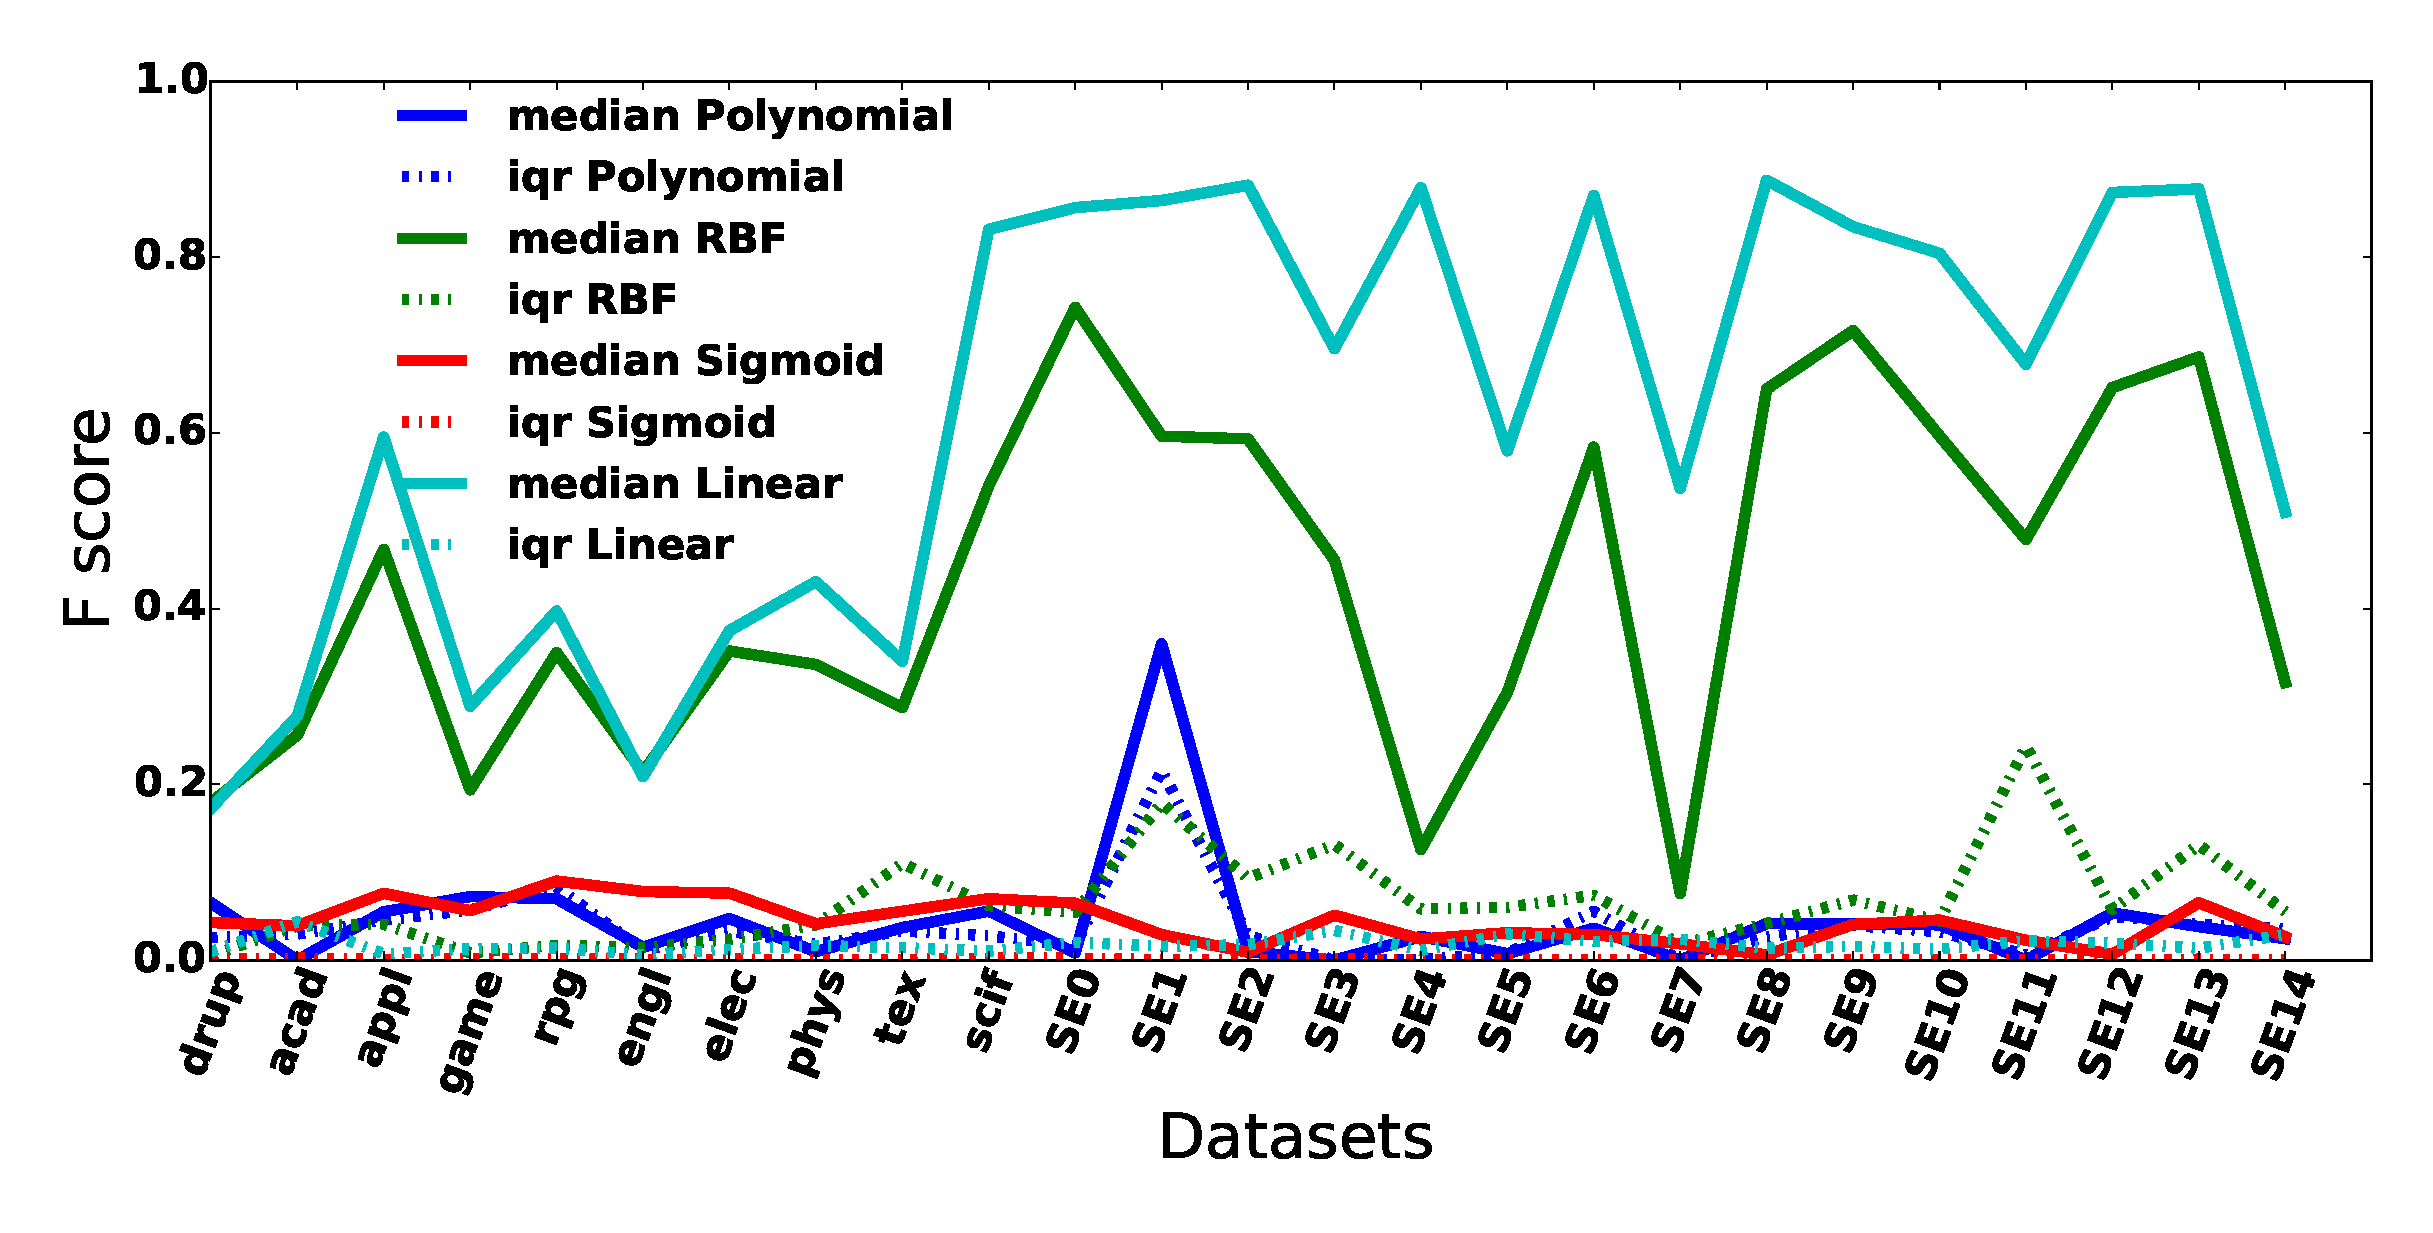
\includegraphics[width=\linewidth]{./fig/algms2.eps}
%   \caption{Kernels}
%   \label{fig:algms2}
% \end{figure}

\subsection{Best Practice}

According to the result of the above experiments, the setting of our best practice is:

\textbf{Tokenization:} stemming and stop words removal.

\textbf{Featurization:} term frequency.

\textbf{Normalization:} L2 normalization on rows.

\textbf{Dimensionality Reduction:} hashing trick, 4000 features.

\textbf{Data Balancing:} SMOTE as oversampling method and sample without replacement as under-sampling method.

\textbf{Classification:} Linear SVM.

The median value of F scores of the best practice are: $0.78$ on site-level data sets and $0.39$ on tag-level data sets. 

Most of the settings of LexisNexis text miner is validated to be the best choice while we have also detected a promising improvement when having SMOTE as a data balancing method. Figure \ref{fig:balance} compares our best practice with LexisNexis setting and as discussed in \tion{Data Balancing}, SMOTE has a significant improvement on the performance. The LexisNexis team has already working on adding SMOTE into their products. 


\section{Discussion}
\label{sect:Discussion}


\textbf{Complicate methods may not perform better. }Each preprocessing method described above in \tion{Experiment} has different computational cost. The surprising fact is that the single-parse preprocessing methods - stemming and stop words removal, term frequency, hashing trick, and L2 normalization on rows perform better, or at least no worse than their multi-parse competitors. It may not be true for all data, but this implies that sometimes simple is better.

\textbf{CPU farm is important to validation tasks.} The whole experiment has 25 repeats of 22 different settings on 25 data sets, which counts up to 13750 times of training. We distributed the tasks to 75 computing nodes with 6 or 8 processors per node on a HPC Cluster provided by NC State University. The total runtime is up to three hours and we can expect a hundred times slower if running on a single processor.

The results highlights why these need to be repeated. Certain standard text mining practices are not always useful. When using such practices for big data, it becomes important to choose faster techniques to reduce the computational load. 

\section{Validity threats}

There are several validity threats to the design of this study. 

\textbf{a)} Limited number of text mining decisions are explored, which cannot represent the whole decision space. 

\textbf{b)} Greedy search is conducted in our validation process, which can only prove that the best practice we get is of local optimal, other than of global optimal. 

\textbf{c)} data we use are exactly the data LexisNexis use. For LexisNexis data, the cost of human efforts does not allow a $20\%$ as  training samples, instead, only a thousand of training samples can be used. Therefore semi-supervised learning such as active learning must be included in the approach.


\section{Future work}

%\textbf{RQ4} How can we further improve the performance?

\textbf{Explore more.} Zhe and Amritanshu are involved in literature review for the further exploration in larger space.

\textbf{Cost effective tuning.} In order to explore a larger decision space as well as avoiding local optimum, heuristic search algorithms such as differential evolution, GALE, and NSGA-II will be applied to tune the decisions for a better approach \cite{storn1997differential,krall2015gale,deb2002fast}. We are working on this to achieve both less number of comparisons and better solutions.

\textbf{Active Learning.} Recursive active learning will be introduced to reduce the number of training samples needed. Instead of 20\% of the data, only a thousand samples will be selected and then used for training. The performance of prediction will rely heavily on how representative the selected samples are, and active learning is the key method to achieve it \cite{tong2002support}.





\section{Conclusions}
\label{sect:Conclusions}






 

%
% The following two commands are all you need in the
% initial runs of your .tex file to
% produce the bibliography for the citations in your paper.
 \renewcommand{\baselinestretch}{0.9}
\bibliographystyle{abbrv}
\small
\bibliography{sigproc}
\balance
\renewcommand{\baselinestretch}{1}

 % sigproc.bib is the name of the Bibliography in this case
% You must have a proper ".bib" file
%  and remember to run:
% latex bibtex latex latex
% to resolve all references
%
% ACM needs 'a single self-contained file'!
%
\end{document}
